\documentclass[12pt]{report}
\usepackage{amsfonts}
\usepackage[utf8]{inputenc}
\usepackage[T1]{fontenc}
\usepackage{lmodern}
\usepackage{suthesis-2e}
\usepackage[font=small,labelfont=bf]{caption}
\usepackage{comment}

\doublespacing

\usepackage{amsmath}
\usepackage{amsthm}
\newtheorem*{definition}{Definition}
\newtheorem*{claim}{Claim}
\newtheorem*{theorem}{Theorem}
\newtheorem*{corollary}{Corollary}
\newtheorem*{lemma}{Lemma}
\newtheorem*{property}{Property}

%\usepackage[nottoc]{tocbibind} %Adds "References" to the table of contents
\usepackage{cite}

\title{Background for transient faults in asynchronous circuits}
\author{Zoey Zhou}
\date{\today}  
\usepackage{graphicx}
\graphicspath{ {c:/Desktop/} }


\begin{document}
\chapter{Introduction}

Faults in digital circuits arise from sources such as fabrication defects and radiation.  These faults can ultimately lead to failures of the component.  Thus fault tolerant designs are crucial especially in applications where errors can have disastrous consequences such as in aviation or banking.  Moreover, due to new technology and shrinking transistor sizes for MOSFETs, radiation effects become more prominent.  Because designing fault-tolerant circuits is such an important problem, there has been significant previous work done on fault-tolerance for synchronous circuits.  However there are less work done on fault-tolerant asynchronous circuits.  The research described here aims to fill that gap.\\

Asynchronous circuits differ from synchronous circuits in that the gates have arbitrary delays so asynchronous designs must be more meticulous to account for these delays.  The arbitrary delays also make fault-tolerance a harder problem.  For example, the classic solution of Triple Modular Redundancy (TMR) does not work for asynchronous circuits.  The main contribution of this work is proposing a new fault-tolerant design for asynchronous circuits.  The new design expands fault-tolerance to semi-modular speed independent circuits composed of two-input gates and C-elements.  This work also proves that the proposed fault-tolerant design is tolerant to transient faults.  With this new design, circuits can be more robust to different types of errors, allowing the circuits to be used in a greater variety of environments.



%Digital circuits is the basis of many of present day electronics.  Digital circuits has signals which are represented as discrete values.  This is achieved by choosing a range of voltages that correspond to each discrete value.  Many digital circuits use binary values, that is the signals can only take on the value `logic 0' or `logic 1' (or low/high).  One advantage of only allowing discrete values is that digital circuits are much more robust to noise fluctuations in voltage.  Disregarding the lower level implementation, one can also abstract the function of digital circuits in terms of gates.\\

%Although digital circuits are less sensitive to errors due to noise, it can experience other faults in its electronics which ultimately may lead to failure of the component.  Faults may arise due to fabrication defects and radiation such as from space.  Moreover due to new technology and shrinking transistor sizes for MOSFETs, radiation have caused more noticeable effects even at sea level. Thus designing fault free circuits is an important problem to study and solve.  \\  %can still be expanded

%This work focuses on a class of digital circuits known as asynchronous circuits.  There is an arbitrary delay on the gates of asynchronous circuits so that each design must be additionally verified to operate correctly under such delays.  There is a variety of uses of asynchronous circuits because it has speedups over synchronous circuits and is also useful for synchronous systems where there is significant clock skew or combining components with different clock cycles and/or interfacing with the real world.  There are some previous work that has been done to make asynchronous circuits fault-tolerant to soft errors.  The design is based on duplicating the circuit and only works for quasi-delay-insensitive circuits which requires a lot of assumptions about how the delays in the underlying transistors function.  The main contributions of this work are that it extends the previous work by proposing a new design.  The new design also follows the duplication strategy but makes fault-tolerant the class of semi-modular speed independent circuits (a class of circuits about the same size as QDI circuits) with looser assumptions on the delay and without significant overhead.  Namely the only assumption is that the combinational logic components are composed of gates and that each gate is allowed to have arbitrary delay, instead of assuming that there is no delay in these components.  Previous designs do not work for this more generalized case of circuits.  This work also proves that such a fault-tolerant model will always work and correct transient faults.  This allows for circuits to be more robust to different types of errors that may occur and prolong the lifetime and types of environments this circuit can be used for.

\section{Synchronous vs Asynchronous circuits}
Digital circuits can be divided into two types, synchronous and asynchronous.  The time it takes for gates to process input signals and then propagate the output to the next gates in a digital circuit may vary widely.  If the timing is somehow off, it is possible for the outputs to be different from the desired value resulting in incorrect computation. In synchronous systems this timing variation is dealt with by using a global clock.  The clock is then fed into each flip flop so that the flip flop outputs will lock and update the signals synchronously. The clock cycle frequency is chosen so that all of the gates can finish processing and the correct values are locked for the next cycle. That is, the clock cycle is usually designed to accommodate the slowest logic element. The design of synchronous systems can be complex and is not necessary to understand in detail for this work. \\
\begin{figure}
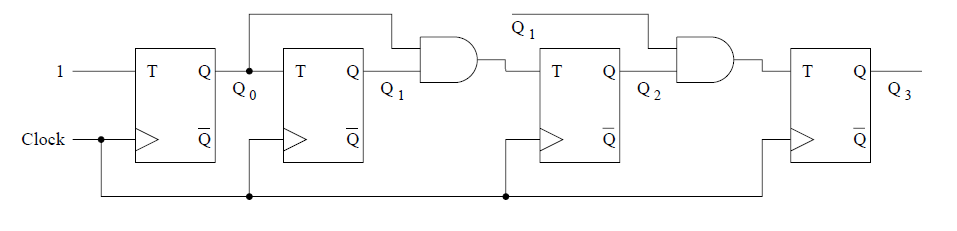
\includegraphics[width=\textwidth]{syncex}
\captionof{figure}{Example of a synchronous digital circuit.  Each output is gated by a flip flop that is controlled by the clock}
\end{figure}
%possible picture of clock and flip flops?.... redraw as my own

Asynchronous circuits, as the name suggests, do not depend on a clock. As a result there are varying time delays in their components. The goal of designing asynchronous circuits is to make circuits that achieve some specification in spite of the time delays. That is, irrespective of the time delays, the circuit meets its specification. One main reason that asynchronous circuits are used is that they do not require clocks to propagate signals; instead as soon as one logic element finishes the signal goes directly to the next element.  This can allow the circuits to have speedups as it is not waiting for the slowest element for each clock cycle.  The resulting circuit is also very robust as it already accounts for possible variations in manufacturing that contribute to varying time delays.  Additionally even in synchronous systems, small asynchronous circuits are needed to match the inputs coming in from different circuits with different clock frequencies or from the outside world.  For large synchronous circuits, clock skew from different parts of the system is also an issue and may be solved with asynchronous methods. \\ %Martin did not give references for these....prob ok then

\includegraphics[width=\textwidth]{}
\captionof{figure}{Example of a simple asynchronous circuit.  Note that there are no clocks and the signals can propagate at any time}

However, because the signals can arrive at the input at any time, the design is more complicated to ensure that the entire circuit functions correctly.  From a high level view the circuits are designed so that the signals progress irrespective of the delays.  This property is called Delay Insensitivity or Speed Independence depending on the underlying delay assumptions such as the maximum length of delays and on which components.  Even if this is designed correctly, when implemented there can still be hazards.  A hazard is when a certain sequence of delays of the circuit cause unwanted signal transitions to occur.  This may then propogate to other parts of the circuits and cause unwanted behavior.  When trying to eliminate hazards, the underlying delay assumptions are important as well as the implementation details such as gates and transistors. Given the same design under one implementation the circuit may have hazards while under another implemention the circuit will be hazard-free.  Some of the different delay assumptions that could be made are that the delays only occur at gates, or delays only occur on the wires or the delays occur on both gates and wires \cite{myers_book_2004}. Furthermore the bounds on the delay can vary as well. The most stringent case is if we assume that the delay can be arbitrarily long and takes on a value anywhere in the interval $(0,\infty)$ \cite{myers_book_2004}.  Circuits built under the unbounded gates and wires delay model are called Delay Insensitive circuits.  We will not use this delay model because the class of Delay Insensitive circuits is very restricted.  In particular one can only use buffers, inverters, and Muller C-elements to build Delay Insensitive circuits \cite{Martin_1990_DI} \cite{Martin1986_DI}.\\ %2nd reference not necessary 

The asynchronous delay model that we consider is the unbounded gate delay model.  Circuits that can handle any delay under this model are called Speed Independent circuits. The unbounded gate delay model assumes that delays only appear on the gates and the delays can be arbitrarily long in the interval $(0,\infty)$.  The wire delays are negligible.  In addition we assume all forks, which is splitting a signal into multiple branches, do not have any time delays between each of its branches.  These assumptions are reasonable because the delays on the wires only change the operation of a circuit if the wire has forks.  (Otherwise you can lump the wire delay with the previous gate)  When a wire has forks, it is usually true in implementation that the delay between different branches of the fork is less than the delay for gates so that they arrive at the next gates at the same time from the perspective of the relevant gates.  This is also termed isochronic forks.  We focus on the unbounded gate delay model because the delay being unbounded is a pretty harsh requirement and would allow more circuits to work in a real life setting. \\ %how if we assume both gates and wires have delay cannot create many SI circuits, and also Muller is one of the broader classes that we can use

D. E. Muller proposed essentially this class of speed independent circuits, which are sometimes called Muller circuits \cite{Muller_59}.  Since then a number of synthesis methods following this design has been produced.  Usually the synthesis methods begin with some higher-level specification such as a signal transition graph or Petri net and translate into a state graph.  A state graph describes all the possible sequences of changes in a finite number of signals.  (The term wires and signals are used interchangeably as the state graph is converted into a circuit.)  Then depending on the underlying implementation, such as generalized C-element and standard C-implementations, the appropriate inputs and logic functions that allow the circuit to function according to the state graph is synthesized.  The end result is a hazard-free and speed independent asynchronous circuit.  The construction we describe begins with a semi-modular circuit, possibly resulting from the previously described process, and transforms it into a circuit that can tolerate any single transient fault.
     
%There are other types of delay models and asynchronous circuit synthesis methods such as Quasi Delay Insensitive circuits and the relevant types for this work are described in more detail in the literature review.  \\  %add refs to gen C etc

\section{Organization of this work}
%why are async circuits important, timing delay etc
Because these various faults can interfere with the function of the circuit and even result in harmful operations (catastrophic failures), there has been a lot of work on making digital circuits fault-tolerant. Most of the fault-tolerant solutions have been investigated for synchronous digital circuits.  Because the timing difference between different signals arriving do not have to be considered for synchronous circuits, they can use error correcting codes and redundancy techniques such as triple modular redundancy (TMR). Unfortunately most of these techniques are not applicable to asynchronous circuits.\\

In this work, we propose a new fault-tolerant circuit transformation on asynchronous semi-modular control circuits.  We also propose a method of comparing the fault-tolerant circuit with the original circuit, by comparing traces with the half circuit.  The fault-free half of the fault-tolerant circuit behaves like the original circuit under single transient faults.  In addition, we assume a gate-level model of the circuit and allow the transient to occur on any of the wires thus solving the transient fault problem for a bigger class of circuits than the current state-of-the-art.\\

The rest of this work is organized as follows.  Chapter two introduces the different types of common faults and their causes, as well as the common fault models that researchers use when investigating these faults.  Also included in chapter two are the asynchronous circuit models that are relevant to this work.  In addition, there is discussion about the existing body of work on fault-tolerant solutions for both types of circuits with an emphasis on asynchronous circuits.  Chapter three provides the background concepts and definitions for asynchronous circuits.  Chapter four shows why the existing fault-tolerant methods are insufficient and propose a new fault-tolerant method for asynchronous transient faults.  We prove the correctness of the method using a combination of automated formal verification and manual methods.  And finally chapter five discusses how to better build fault-tolerant asynchronous circuits and suggests some possible new research directions.
%Overview:  why is the problem important  \\  maybe I can extend the Introduction a bit more

\chapter{Related Works}
\section{Faults}
Faults can be split into permanent and non-permanent faults. Non-permanent faults are further split into transient and intermittent faults \cite{jha_gupta_2003}. %copied 
A fault is defined as the physical difference between the good or correct system and the current system. An error may be caused by a fault, which is when the state of the system differs from the state of the good system and thus unable to perform some specified function. Hidden faults are also possible where the fault does not cause an error \cite{jha_gupta_2003}. \\

Permanent faults refer to the presence of a fault that affects the functional behavior of a system(circuit) permanently. Some examples that may cause permanent faults are: incorrect connections between integrated circuits, broken components or parts of components, incorrect silicon and metal connections (manufacturing problem), and functional design errors. Most permanent faults occur during fabrication. There are many existing literatures that cover permanent faults and the different tests at production time that can uncover the presence and location of these faults. \cite{jha_gupta_2003} \cite{giz_book_2006}. We ignore the possible manufacturing problems and assume that the circuit is free from those problems. Instead we consider the permanent faults that develop during operation from radiation. For example, high energy ions can impact the transistors and the circuit causing short-circuiting, rupture of the gate oxide insulation and other permanent faults.\\ %copied from SEE eetimes article

Non-permanent faults are defined as faults that affect the system's functional behavior for a finite but unknown period of time. They can occur at random moments and are categorized into two types, intermittent and transient faults. Intermittent faults are caused by non-environmental conditions such as loose connections, deteriorating or aging components, critical timing (hazards and race conditions), resistance and capacitance variations (which may lead to timing faults), physical irregularities, and noise. Intermittent faults usually affect the system for a shorter time period than the application time of a test developed for permanent faults and thus may not be detected using such a test. Intermittent faults can transition into permanent faults naturally but may take a long time from hours up to months. \\

Transient faults are caused by environmental conditions such as cosmic rays, $\alpha$-particles, pollution, humidity, temperature, pressure, vibration, power supply fluctuations, electromagnetic interference, static electrical discharges, and ground loops. In particular $\alpha$-particles are a major cause of these faults. These $\alpha$-particles can interact with the semiconductor material which results in the generation of electron-hole pairs. When these $\alpha$-particles collide and interact with the circuit it can induce a voltage/current pulse. Also known as single-event transients (SETs), if the width of this pulse or transient is wide enough it may propagate through the circuit. $\alpha$-particles may also interact with a memory element (of which flip flops, latches and C-elements are most relevant to this work) and cause a bit flip in the state of the memory element. This is also known as single-event upsets (SEUs), SEUs include both single-bit and multi-bit upsets but single-bit upsets are most common and much work has been done to eradicate failures from SEUs. 
Transient faults may be hard to detect because it appears sporadically and may not affect the system during testing. \\

In this work we will not be concerned with intermittent faults since it can be thought of as a transition between transient to permanent faults. Instead the two main fault modes we will look into are transient and permanent faults. In both radiation effects, also called single event effects (SEEs), figure prominently. SEEs are an umbrella term that covers the aforementioned SETs and SEUs as well as the single event effects causing permanent faults. There are two main sources of radiation, one is cosmic rays from space which interact with the atmosphere to produce high energy neutrons. Another is that $\alpha$-particles can be caused by trace impurities of radioactive elements present in the packaging material of the chip and the silicon substrate. Radiation from cosmic rays become more severe at higher elevations while the latent source in packaging is difficult to eliminate. Thus, initially a lot of the work in fault-tolerant design was done for aviation and space flight.

%failure mechanisms - physical and electrical causes of faults% maybe not that useful... may not need to go in depth

%digital circuits
%Types of faults transient/perm (and possibly subcases too) \\
%Asynchronous circuits (different types) possibly synchronous too? (and our circuit model based on Meyer) \\
%Then talk about the fault-tolerant solutions () \\


\section{Asynchronous Circuit and Synthesis}
In the previous chapter we described how an asynchronous circuit works from a higher-level perspective and in particular that it should work under varying delays. In this section we will cover some definitions and properties of the circuit and also how we can synthesize the circuit from a higher-level specification. Both Speed Independent and Delay Insensitive technologies will be introduced. There are differences but also many similarities between the two methods. Even though this work is based on the Speed Independent model, there has been some previous work done on the Quasi-delay Insensitive model so I wanted to provide some context to make a direct comparison.

\subsection{Speed Independent Circuits}
As mentioned in the introduction, circuits are composed of gates and wires. The unbounded gate delay model assumes an arbitrary delay on all the gates and no delay on wires. This delay model is the basis for Muller circuits \cite{Muller_59}. Circuits that operate correctly regardless of the delay are called Speed Independent Circuits. The correct operation is specified when designing the circuit, for example, given some input values the circuit will return specified output values. 
There are many ways to represent specifications such as Petri nets and state graphs, and there are established methods to build asynchronous circuits to satisfy the specifications. We won't go into these representations and methods in detail, other than the aspects that are relevant to this work. We consider circuits which has wires that take on Boolean values of either `1' or `0'.\\
%Wires in the circuits take on Boolean values of either `1' or `0'. A state is defined by assigning a Boolean value to each wire of the circuit. States are unique in that no two states share the same wire values. There will be a formal definition of wires and states in the next chapter.

\begin{comment}
State graphs describe how we would like the circuit to function. 
Muller circuits are then synthesized from the state graphs.
\begin{definition}A state graph consists of $\langle W, S, T\rangle$ where $W$ is the set of finite signals $\{w_1 .. w_n\}$. $S$ is the set of functions $[W \to \{0,1\}]$ %<-this might not be right math... and s(k) denotes the (binary) value of the state at signal $v_k$. 
which maps each variable to a boolean. An element of $S$ is called a {\em state}. $T$ is the transition relation of the state graph, $T \subseteq S \times S$. \end{definition}

State graphs can also be thought of as each state having a boolean value for each of the signal variables, and states can be named by these values. For the state graphs that we work with, we assume all states are distinct and that in each transition, only one of the signal values change. The transition arrows are usually labelled with the signal variable and in which direction the change occurs to help with an easier understanding of the graph. 

\includegraphics[width=\textwidth]{stategraphex}
\captionof{figure}{Example of a state graph. The order of the variables in each state are x,y}
State graphs can be implemented as an asynchronous circuit where the signals of a state graph $V$ maps one-to-one to wires in the circuit. Then the set of states $S$ can also describe the state of wires of the circuit. \\

Next, we describe the set of {\em transitions} of a circuit where only one signal value changes more formally. 
We write $s(w)$ for the value of signal $w$ in state $s$, and write $T(s, s')$ when there is a transition from $s$ to $s'$.

A transition has the additional constraint that only one signal is allowed to change between the two states in the transition:
\begin{property}For all $s$ and $s'$ in $S$, whenever $T(s,s')$ holds, there is exactly one $w \in W$ such that $s(w)\neq s'(w)$.
\end{property}
There may be multiple transitions from a state $s$. A related concept is when the state of a circuit changes when one or more circuit elements is unstable, leading to a change in its output signal. An unstable element is said to be {\em excited}.


\begin{definition}A wire $w$ in the circuit is {\em excited} in state $s$ if there exists a $s'$ such that $T(s,s')$ and $s(w) \neq s'(w)$. % Alternatively we define a function $f_v$ for wire $v$ such that if wire $v$ is excited in state $s_i$ then $f_v(s_i)$ takes on the value after the excited wire transitions and $f_v(s_i)\neq s_i(v)$. If wire $v$ is not excited then $f_v(s_i)= s_i(v)$. 
\end{definition} %delete second part if I don't use f_u() later
%For example we propose $f_s$ and $f_r$ as functions that maps the current state to the output of the set and reset blocks respectively.
%(may need to change this definition to s'=/=s) <- added in

Note that from a state $s$ it is possible for multiple wires to be excited as defined above because there may be multiple transitions from $s$ to different states. Each of the transitions causes a different signal to change.
%[Explain that multiple elements can be excited in the same state because there can be transitions to several different states, and each of those transitions can change a different signal.]
%[Think about including examples: a boolean gate and a C element ]

We consider semi-modular circuits because they are a subset of speed independent circuits and is a large enough class to include some interesting and useable circuits. A simple explanation of semi-modularity is that once a wire is excited, it stays excited until it transitions to the excited value. Formally this can be defined as follows: %proof that semi-modular circuits are also speed independent
\begin{definition}An asynchronous circuit is {\em semi-modular} if for every pair of states $s$ and $s'$ such that $T(s,s')$ holds, and let $v$ and $w$ be wires such that $s(w) \neq s'(w)$ and $w\neq v$, then if $v$ is excited in state $s$, $v$ is also excited in state $s'$ \end{definition}

%ADD SPECIFIC CONDITIONS THAT ALLOW SYNTHESIS
When the state graph has the following properties, it is possible to synthesize a hazard free and speed independent asynchronous circuit following the state graph. Each variable from the state graph is implemented as a gate logic that takes other variables/wires as inputs and outputs a variable/wire. We next look at how such a gate logic can be made.\\ 
\end{comment}


%C-elements
The C-element proposed by Muller is an important building block for asynchronous circuits. It acts as a memory element in that it receives two inputs. When both inputs are low, the C-element output goes low, and when both inputs are high the C-element output goes high. However, when the inputs are mismatched then the output gets held at its previous value. This can be achieved in a number of ways such as a gate implementation as well as a transistor level implementation with feedback using a weak transistor, other implementations use capacitance to achieve this weak feedback.
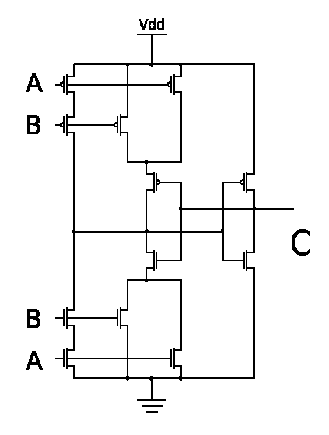
\includegraphics[width=\textwidth]{celement}
\captionof{figure}{a. logic of the C-element. A, B are inputs, C is the output \\ b. diagram of a C-element at the gate level c. transistor-level implementation}

C-elements can be used in various asynchronous circuit designs and is an essential component of Muller circuits. \\

The two specific Muller circuit implementations that we consider are the generalized C-element and standard C-implementations. We assume that the circuits we want to make fault-tolerant are synthesized according to these two implementations. 
Each wire in the circuit is the output wire of a gate logic. The gate logic has a set of input wires and the output wire changes value according to the values of the inputs. We look at two conditions, set, the condition for the output wire to transition to a high value; and reset, the condition for the output wire to transition to a low value. The gate logic then implements the set and reset conditions. 
We skim the details in finding the set and reset conditions from the circuit specifications. For each condition set and reset, there is an ON-set, OFF-set and Don't Care set. ON-set are all input values where the wire is excited and a transition will occur. The OFF-set includes all input values where the wire cannot be excited to some value per the circuit specifications. Input values that are neither in the ON-set or OFF-set are in the Don't Care set. So, for the set condition, the ON-set are all input values where the wire must transition to high. The OFF-Set includes all input values where the wire is excited instead to low, as well as input values for which the output wire must remain low. The input values of the Don't Care set assign the output wire to be either high or low. It does not matter which value is assigned since it does not disturb the function of the circuit and only helps for circuit optimization. \\

The same procedure applies as well in finding the ON-set, OFF-set and Don't Care set for reset except substituting in reset for set and flipping the value of the wire from high to low and vice versa. The set and reset conditions constructed this way then follows the desired circuit specification. The set and reset conditions are implemented using gates and are combined into the output wire through a C-element. This entire block of gates and C-element for the output wire is called the gate logic. \\ %Beerel and Myers.... also expand? 

Even though the generalized C-element is presented as a C-element with set and reset as inputs, the transistor level implementation differs slightly. We assume a transistor level implementation of the set and reset combined with the C-element so that there is only one delay for the entire logic block. In addition, this is not a normal C-element because set is used exclusively for the pull-up logic and reset is used for the pull-down logic. In a normal C-element we allow for any four combinations of the values of the set and reset input wires. However, using the pull-up and pull-down logic setup, we do not allow for when both set and reset is `ON' as the output wire would simultaneously be connected to the high voltage and ground. Such an output would have indeterminable voltage values and violate the digital assumptions. Thus, the set and reset logic is designed so that they cannot overlap. This corresponds to $\overline{set}\vee\overline{reset} $ is always TRUE.\\
\begin{center}
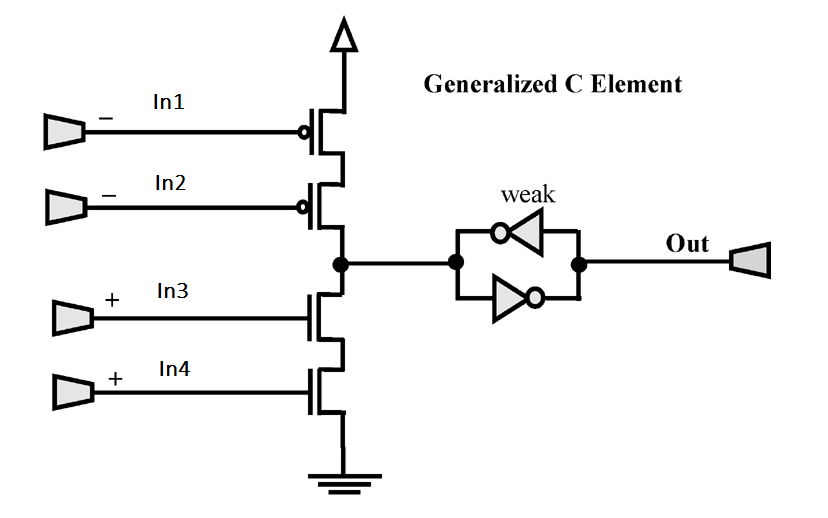
\includegraphics[width=.7\textwidth]{genC}
\end{center}
\captionof{figure}{transistor level implementation of a generalized C-element. The + signs are the set logic inputs and - signs are the reset logic inputs. For this particular element, set is in3 AND in4 while reset is in1 AND in2.}

The main difference is that the set logic and the reset logic must be designed so that they do not turn `ON' at the same time.\\

For the standard C-implementation, we allow for more variation in delay. For each wire in the circuit with a corresponding gate logic, we look at the set and reset logic as composition of various gates (such as AND, OR, NOT). Each of these gates can have their own delay that is arbitrary in length that is instantized as an intermediate wire. Thus, the logic must be synthesized more carefully to eliminate hazards that can occur in these intermediate wires. In particular the set and reset must be activated at states only when the wire is appropriately excited. As a result, the standard C-implementation has a number of set logic functions combined by an OR gate and fed into one input of the C-element. There will also be a number of reset logic functions combined by an OR gate and passed through an inverter and fed into another input of the C-element. This implementation uses the standard C-element so that if the set and reset inputs are mismatched, the output is held. In general, the synthesis can be changed so that there is a hazard-free implementation using only two-input gates.
%explain sop?
\subsection{Quasi Delay Insensitive Circuits}
%QDI
Quasi Delay Insensitive Circuits (QDI) are related to Delay Insensitive Circuits. Previously we mentioned that Delay Insensitive circuits operate under the assumption that both the gate and the wire have unbounded gate delays. In particular each branch of a fork will have different delays and can be treated as separate wires. One result about Delay Insensitive circuits is that it is a very restricted class. Instead if that condition is relaxed so that some of the forks are allowed to be isochronic, then a more general class of circuits can be constructed. Note that in the case where all forks are isochronic, then this becomes the same as speed independent circuits. \\
The gates of a QDI circuit is formed from Production Rules (PRs). For the single output case, a gate takes a set of variables as inputs and outputs a variable. Again, a transition on the variable $x$ is denoted as $x\uparrow$, a transition from $x=0$ to $x=1$; and $x\downarrow$, a transition from $x=1$ to $x=0$. Then the two PRs associated with the gate with output $x$ is :
\begin{align*}
B_u\mapsto x\uparrow \\
B_d\mapsto x\downarrow 
\end{align*}
Where $B_u$ and $B_d$ are called guards. Each guard is a boolean condition formed by some combination of the input variables. When a guard is evaluated to be $True$ then the transition is activated. When it is $False$ then the corresponding transition does not happen. Note that similar to the generalized C-elements, both guards cannot be active at the same time. In addition, it is assumed that each guard is in a sum of products of the input variables. The PRs of a circuit are evaluated all at the same time. At any point in time, if a transition is activated, it will transition in a finite amount of time as long as the corresponding guard is held at $True$. This is due to the assumption of the arbitrary delay of a gate. Note that again, like the generalized C-element implementation, we assume that the transistor level implementation of a PR allows any arbitrary sum of products to be made where there are no delays within the logic of the sum of products.\\

Another important property of QDI circuits is \textit{stability}. A guard is stable if it evaluates to False after the transition of the output variable is complete. This eliminates any hazards that may arise when a guard is True and before the output has fully transitioned, the guard then evaluates to False and the transition is terminated. This may cause a blip in the voltage, an incomplete transition, where the circuit may interpret it as either no transition or two consecutive transitions. One additional assumption is that the PRs cannot be \textit{self-invalidating}. That is, when a transition on an output occurs, it cannot immediately falsify the guard. With this assumption, it can be shown that the output of a gate cannot also be its own input variable. There are no self-loops. 

\section{Fault Tolerant solutions}

%soft error protection <- error correcting codes for SRAM memory
Because faults cannot be eliminated in digital circuits, different methodologies have been used to make the circuits fault-tolerant. Much of the research done in this area are for synchronous circuits. There has also been some research for asynchronous circuits using some similar techniques. First, we present an overview of some common techniques for synchronous circuits, then introduce the current techniques for asynchronous circuits. Some of the techniques in asynchronous design borrows or are inspired by the much more developed fault-tolerant synchronous circuits field. However due to the difference in timing assumptions of the two types of circuits the techniques are not completely transferable. We describe why some of the solutions from synchronous circuits cannot be directly applied to asynchronous circuits.\\

%- used in the early days for space and flight, and systems that CANNOT go offline/errors like stocks and banking.
%- different techniques... explain a bit about each
%-hardware, software, hybrid, 
%-detection vs correction
%- ECC/ parity checking (needs software/ controller) (Mitra's method)
%-TMR is still super important (possibly why TMR is not viable for async)
In the early days there were certain systems for which eliminating faults and errors were very important. These include space and aviation control systems where due to the altitude there are more radiation and thus more faults. In addition, faults that cause error is very detrimental to these systems and may cause failures leading to loss of life. Other examples of systems requiring reliable circuits include banking and stock market applications where the system must function without error for hours at a time and in case of any error may have devastating consequences, such as a bit flip of the most significant bit in a money transaction. \\

Solutions for eliminating these transient fault-induced errors include physical, hardware, software or a mix of the previous. Some commonly used techniques are transistor sizing, circuit hardening, hardware duplication, and time redundancy \cite{Mitra_08_softerrors}. Transistor sizing is a physics-based technique and does not reduce as much soft errors as the other techniques. Circuit hardening is on the physics level, where it uses intrinsic properties such as resistive or capacitive hardening, or combining the transistors differently to have less effects from transient faults. (?) Hardware duplication, is a common technique that tries to eliminate soft errors on the circuit level. This is achieved by having multiple duplicates of a circuit and often comparing the value from each duplicate to find and eliminate errors. For example, Triple Modular Redundancy (TMR) has been used since the beginning of the field and is still a good solution for eliminating single soft errors. The advantages are that it is able to eliminate nearly all soft errors but also due to the duplication, the area for each circuit and additional power increases substantially (correlates to the number of additional duplicates). Time redundancy techniques re-use the same circuitry to compute values multiple times to ensure there is no error. This technique is not completely hardware based and requires software to manage re-using the same circuity with the same inputs over time. The area of the circuit does not change but the speed of the circuit worsens substantially. \\

There is also the additional distinction between error detection versus error correction. In general, it is easier to detect an error than to correct it. For example, using hardware duplication, only 2 copies are required to detect an error but 3 copies (TMR) to correct the error. For different parts of the system there are also different strategies. For example, in memory components such as SRAM, soft error correction is usually done using error-correction codes. These codes are compared to the bits that are stored to ensure that there are no errors. They are designed to handle a predefined maximum number of errors. For example, Hamming codes where each codeword are at least a distance of 3 apart can handle one error. This method is not purely hardware based and a controller system and software are used to match the codes and detect and correct any errors. For a control circuit, there are also a variety of strategies. Again, one could make use of error correcting codes or parity bits to detect or correct errors in combinational logic \cite{McCluskey_99}. This uses a combination of hardware and software. A completely software approach is to run a program on some input, then run the program again on a transformed version of the input where the output can be mapped back to the original output \cite{Mitra_softwareerror}. If the output and the transformed output do not match then the fault is detected. Lastly, for hardware only methods, even now TMR is a commonly used method because of its robustness and ensures error correction. \\
%However these cannot be used for latches or flip flops. In these circuits, some of these techniques only detect errors but do not correct them.\\

Triple Modular Redundancy is a technique where each combinational logic unit is copied three times and then fed into a latch that performs a majority voting operation. That is, if at least 2 out of the 3 signals agree on a value, the output becomes that value. Additionally, to counter possible faults on the single output wire, the majority vote unit can also be copied three times and its output wire fed appropriately as input to the three copies of the downstream combinational logic. This would resolve both transient and permanent single faults. However, the downside is that the circuit needs to be copied three times so the area is three times larger and the power consumption as well. In addition, there must be many adaptations for this to work in asynchronous circuits as the signals can arrive in different orders. We give an example of why TMR does not work in an asynchronous circuit as it does in a synchronous circuit below. We assume that in the original circuit that each logic block has some input wires and an output wire. In the TMR scheme, each logic block is triplicated and to remove single points of failure, we also triplicate the majority voter that the three copies of the output wire feeds into. There are also three distinct copies of each input signal that correspond to outputs from the three voters. This is the basic scheme that synchronous circuits with TMR uses. Because this circuit is asynchronous, we assume that each logic block is composed of gates that has some arbitrary delay that is independent of other gates. This is true under both delay assumptions of speed independent and delay insensitive circuits. We ignore whether a fault can be in the voter for now. 
\begin{center}
\includegraphics[width=\textwidth]{tmrcounterex}
\end{center}
\captionof{figure}{An example of an error if a fault occurs in an asynchronous TMR circuit}
Initially all output wire values are `0's. Then since the input signals are distinct copies of each other, it is possible for one set to finish transitions (new) before the other two sets and the first logic block transitions to a `1'. Then a transient fault arrives on the output of the second logic block which transitions to a `1' as well. The majority voter would then transition to a `1'. However, the upset from transient faults usually happen within a short time period and the old inputs eventually force the output of the second logic block back to `0'. Then the majority voter would transition to a `0' so that causes a hazard on the output of the majority voter. %depends on if the logic gate was combinational logic.... which I guess we can assume it is
%NEEDS FIXING AND CHECKING
It is also possible for the `1' from the majority voter to feed into other logic units which is effectively an early transition. That early transition will then put the circuit into states that are not specified by the original state graph and thus the next states cannot be predicted.
\\

%also included detection schemes because there is so few works in the literature...
David and Ginosar (1995) prove that a specific type of asynchronous circuit called self-timed combinational logic is self-checking under stuck-at-faults \cite{self_timed}. (Stuck-at-faults are permanent faults where a wire value is stuck at 0 or 1) That is if there is a single stuck-at-fault, the circuit will either stall or give an illegal output so that faults can be detected. Each input and output is encoded by 2 bits also known as dual rail encoding. 10 represents 0, 01 represents 1, and 00 represents undefined or the system is not yet ready. 11 is an illegal output that only occurs under certain faults. Each logic unit is composed of four subunits, three of which control the inputs and outputs and includes many C-elements. The fourth one implements the combinational logic. The combinational logic requires the implementation to be such that each output bit is monotonous given the input bits. A further restriction is that the combinational logic is composed of only AND and OR gates.
\\

Verdel and Makris proposes that simply porting the duplication strategy for error detection from synchronous circuits does not work for asynchronous circuits \cite{async_dup_ced}. This is because the duplication strategy relies on both the original and duplicate to output the same value. Some modifications that they propose to make the duplication error detection strategy work is to assume additional timing requirements. That both copies should output the same value within a certain time determined by a pre-set delay element. Everytime one of the signals transitions to a new value, and the duplicates are mismatched the timer starts and if they stay mismatched when the timer ends an error is detected. They look at stuck-at-faults and premature firing faults. There are also cases when the timer detection does not work and for those cases, they propose using additional hardware to look at the states of all the wires to see if an illegal state was reached. They present an example of a control circuit for data computations. The main restrictions of this method are the additional timing assumptions they make about two copies of a circuit, and that the extra hardware components are assumed to be fault-free. Also, it requires an additional comparison unit for each pair of signals which may be costly. Only one copy of the duplicates produces output signals that interfaces with the other units so that if there is an error on that signal it is not detected until some time after the error has propagated.
\\

Almukhaizim and Sinanoglu (2007) propose a Triple Modular Redundancy (TMR) based method of solving transient errors but requires a hazard-free majority voter. Transferring the TMR method that solves faults for the synchronous circuits to asynchronous requires the change that 2/3 copies agreeing is not good enough but 3/3 is needed to propagate a signal. This is due to the asynchronous property where signals can change at any given time and thus one signal changing plus a transient error may cause the output wire to transition prematurely. For permanent errors there is an additional problem of deadlock and this configuration does not solve it completely. \\
\\
In the paper by Manohar and Peng (2005), they add in new circuitry that solves faults for a specific asynchronous adder circuit \cite{PengManohar_asyncadder}. The faults that they consider are fabrication defects, permanent faults and unrecoverable failures. New nodes and edges are added to make it k fault-tolerant. They detect when there is a deadlock at which time it reconfigures the circuit by trial and error of all the possible combinations until the circuit is no longer deadlocked. \\

Naqvi (2014) shows how to solve transient faults on muller pipelines \cite{Naqvi_mullerpipeline}. Muller pipelines make use of handshaking protocols. The assumptions they make are that only one fault occurs per handshake cycle. They used formal verification to show that it works for one pipeline component. \\
\\
Jang and Martin (2005)’s paper considers the problem of single SEUs in QDI circuits \cite{JangMartin_SEUQDI}. In the original functioning circuit, an SEU may cause a) a transition to a deadlocked state, an illegal state with no further possible transitions, b) abnormal, a transition to another state in the state graph and skip or adds certain transitions/signalling, c) tolerant where it transitions to an illegal state but the PRs are unaffected and eventually resumes to a valid state in the state graph. They solve this problem by duplicating the circuit and appending C-elements to the end of each of the original wires. In addition to duplicating the circuit they change the production rule set so that if the rule is about wire $X$ is true in the original circuit, in the new circuit the rule is $X^1$ and $X^2$ both have to be true. For example
\begin{align*}
B_u (...,x,...)\mapsto z\uparrow \\
B_d (...,\lnot x,...)\mapsto z\downarrow
\end{align*}
after duplicating the circuit and adding in C-elements becomes:
\begin{align*}
B_u^{double} (...,x_a\wedge x_b,...) & \mapsto z'_a\uparrow, z'_b\uparrow\\
B_d^{double} (...,\lnot x_a\wedge \lnot x_b,...) & \mapsto z'_a\downarrow, z'_b\downarrow\\
z'_a \wedge z'_b& \mapsto z_a\uparrow, z_b\uparrow\\
\lnot z'_a\wedge \lnot z'_b& \mapsto z_a\downarrow, z_b\downarrow
\end{align*}
The last two production rules correspond to the additional C-elements added. 
They prove that with this new circuit, single SEU errors do not cause transitions to deadlocked states, nor abnormal transitions and thus are corrected. Given the transistor-based QDI assumptions, any changes to the production rules are implemented at the transistor level and assumed to not add any delays. In addition, QDI logic is implemented in sum-of-products form and the production rules are excited only in the appropriate non-illegal states. Faults are assumed to occur on the input/output wires as well as the new wires that feed into the C-elements. Another assumption is every loop in the control circuit is at least length 3 to prevent deadlock. %not sure about this, may only be relevant for when they don't double the inputs
\\

The circuit transformation that Jang and Martin propose work for their assumptions and specific implementation of QDI circuits at the transistor level. However, it is not reasonable to assume that any PR can be implementation with transistors with no delay. Also, for a simple 2-element inverter circuit their transformation also can end up in a deadlocked state after an SEU. After the duplication and addition of C-element. 
\begin{center}
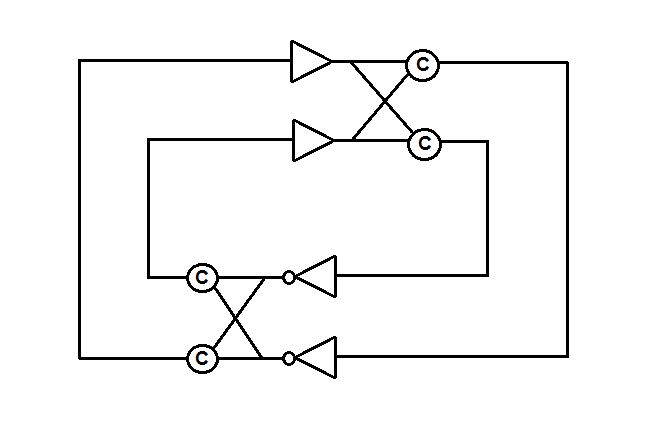
\includegraphics[width=.7\textwidth]{transfex}
\end{center}
Then if a 0->1 SEU occurs at $c_1^B$, it is possible for this circuit to deadlock.
\begin{center}
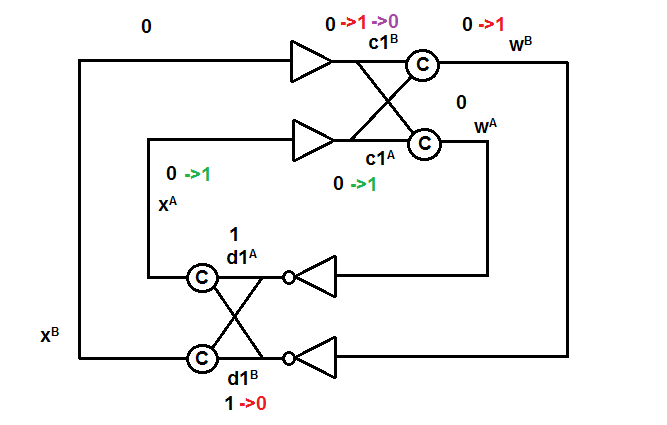
\includegraphics[width=.7\textwidth]{transfexc}
\end{center}
%fix later... it's technically that a simple duplicate and C-element scheme does not work

The approach that we use to make circuits fault-tolerant will be described in the next chaper. Some of the previous works makes additional assumptions such as the checking circuit is fault free or that only one fault can occur on an arbitrarily large transistor gate. We allow for standard two-input gates and assume that all gates in our model are subject to faults. Our fault-tolerant transformation procedure is for a class of circuits, semi-modular control circuits, which includes many circuits.


\chapter{Asynchronous Circuit Concepts \& Definitions}
\section{Assumptions:  Boolean signals}
We make the assumption that all signals are Boolean, that is, the signals are either `logic 0' or logic 1'.  When the the gates and C-elements are excited, and their outputs transition, we assume that transition is instantaneous and that after the transition, the signals are still Boolean.   
Even in cases where the wires are affected by faults, we assume that the new value of the wires are Boolean, and if they are inputs into circuit elements, that the output of the circuit elements also remain Boolean.  For each circuit, there is a finite set of wires, which we call $W$.  An exact definition $W$ will be presented at a later section, but for now just think of $W$ as including all the wires of some circuit.

\section{Notation for Logical Operation}
We use the logical operator notation.  For example, the AND operation with two inputs $w_1$ and $w_2$ is $w_1\wedge w_2$.
The OR operation with two inputs $w_1$ and $w_2$ is $w_1\vee w_2$.  The NOT operation with input $w_1$ is $\neg w_1$.  These are interchangeable with the Electical Engineering convention, which represent AND as $w_1\cdot w_2$, OR as $w_1+w_2$, and NOT as $\overline{w_1}$.

\section{Circuit Elements}
Gates and elements (C-elements) are components that we allow in our circuit.  In general, we call them elements.  Each element has 2 input wires and 1 output wire.  The elements can be in two states, excited or stable.  Examples of gates are AND, OR, NOT etc.

For each element, there exists a function that maps the inputs into a binary value.  This function is represented by $f:[I \to \{0,1\}] \to \{0,1\}$ where $I$ is the set of input wires of the element, a subset of $W$.  If we assume a two input element, we name the input wires $w_1$ and $w_2$.  The function models the designed operation of the element such that if the element had no delay, $f(w_1,w_2)$ is the output value of the element.  With asynchronous delay, if the inputs remain constant, then the output will eventually take the value of $f(w_1,w_2)$.  For gates, such a function is easily defined.  For example, an AND gate such as in figure \ref{fig:gates0} with two inputs $w_1$ and $w_2$ is modeled by the function 
\begin{figure}[h]
\centering
\includegraphics[width=0.4\textwidth]{gates0}
\captionof{figure}{AND gate}
\end{figure}
\[
f_{AND}(w_1,w_2)= w_1\wedge w_2
\]


For C-elements, these are memory holding devices so the function also requires the previous output.  For example, the C-element in figure \ref{fig:element0} with two input wires $w_1$ and $w_2$ is modeled by the function\\
\begin{figure}[h]
\centering
\includegraphics[width=0.3\textwidth]{element0}
\captionof{figure}{C-element}
\end{figure}
\[
f_{C-E}(w_1,w_2) =\left\{
  \begin{array}{@{}ll@{}}
    0, & \text{if}\ w_1=0 \wedge w_2=0\\
    1, & \text{if}\ w_1=1 \wedge w_2=1\\
    v, & \text{otherwise}

  \end{array}\right. 
\]

Each element is in one of two states, excited or stable.  
\begin{definition}
An element with inputs $w_1$, $w_2$, output $v$ and function $f$ is {\em excited} if $v\neq f(w_1,w_2)$.  
\end{definition}
This definition can be extended to include elements with any number of inputs by replacing $w_1$ and $w_2$ with the inputs of a specific element.  A natural extension to an excited element is to consider an element that is not excited.
\begin{definition} 
An element is stable if the element is not excited.
\end{definition}
Then, a stable element must satisfy $v= f(w_1,w_2)$.  An example of an excited and stable AND gate is shown in figure \ref{fig:gates1}.  An example of an excited and stable C-element is shown in figure \ref{fig:element1}.  For C-elements, there are two situations in which the element is stable.  One is where the output is being actively driven to its function value, i.e. when both inputs are 0 or both inputs are 1.  The second is where the inputs are mismatched and the C-element is holding the previous output.  In the second case, the C-element is stable regardless of the output's value.

\begin{figure}[h]
\centering
\includegraphics[width=0.8\textwidth]{gates1}
\captionof{figure}{a) the AND element is excited  b) an excited element fires to become stable}
\end{figure}
\begin{figure}[h]
\centering
\includegraphics[width=0.9\textwidth]{element1}
\captionof{figure}{a) the C-element is excited  b) two types of stable C-elements}
\end{figure}

The states described above are static descriptions of the element, but we must also consider the dynamic behavior.  
That is, when the input or output wires change.  Because we focus on asynchronous circuits, we view these wire changes as happening one at a time with some delay in between.  For example, we do not allow an input wire and output wire to change at the same time.  With this assumption, it is easy to consider all cases for the dynamic behavior of the element.  When the element is stable, the output wire does not change.  A stable element can have input wire changes, and the input changes may cause the element to become excited.  A small point to note is that not all input changes cause the element to become excited, .
When the element is excited, there are two possibilities for the element to become stable again.  Either the input changes such that the element is stable, or the output changes.  Again, not all input changes will cause the element to become stable.  In fact, semi-modular circuits utilizes input changes that allow the element to stay excited.  If the output changes in an excited state, the element becomes stable and we call this action a {\em firing} of the element.

\section{Circuits}
A circuit is a network of elements.  These elements are connected when they share a wire.  For an element, each input is connected to either a primary input or the output of a different element.  Other than elements, a circuit also consists of primary inputs and primary outputs.  Primary inputs are all inputs that are not the output of an element in the circuit.  Primary outputs are outputs of an element in the circuit that connects to another device or element outside of the circuit.  Primary inputs and outputs can be thought of as the interface with outside of the circuit.  They can be the outputs and inputs of a different circuit, or connected to physical mechanisms such as a user pushing a button.   An example of a circuit with primary inputs and outputs is:  .
    
\section{States}
Let $W$ be the set denoting the union of all wires of elements and the primary inputs of a circuit, then $S$ is the set of functions $[W\to \{0,1\}]$ which maps each element of $W$ to a boolean value.  An element of $S$ is called a {\em state}.  

Assigning values to all wires of a circuit names a state.  An example of a state for a circuit containing 3 wires is `101'.  From the set definition, states are unique and no two states share the same values.

\section{Behavior of a circuit}    
Circuits respond to input changes and produces outputs that accomplish some specified task.  Thus the function of a circuit depends on its dynamic behavior and how its state changes over time.  Under the state representation of a circuit, if the value of a wire changes, the state also changes.  If the wire changes from a previous state $s$ to a new state $s'$, then there is a transition relation between the two states.  Defined more formally with $s(w)$ denoting the value of wire $w$ in state $s$:  
\begin{definition}
For all $s$ and $s'$ in S, the \emph{transition relation} $T(s,s')$ holds when there is exactly one wire $w \in W$ such that $s(w)\neq s'(w)$, and wire $w$ must be either the output of an excited element in state $s$, or $w$ is a primary input.
\end{definition}
%from state graph, T(s,s') must satisfy... but we can define ourselves which are the transitions (ie arrows in a state graph).  Going from the circuit, there is a transition if the circuit state allows for a transition, either something excited fires or the primary input changes
There may be multiple transitions from a state $s$.


We define a {\em trace} to describe a path the circuit can take.  Different paths can occur because there may be multiple transitions from each state.  We call the succession of states the trace, which is formally defined as follows:
\begin{definition}A {\em trace} $\sigma=(s_1, s_2, ...)$ of a circuit is a sequence of states of finite or infinite length.  
%Formally this is written as $\sigma: 0,\ldots ,n-1 \to S$ and $n \in \mathbb{N}$.
 Every pair of consecutive states in a trace are in a transition relation $T(s_i,s_{i+1})$, where state $s_i$ represents the $i^{th}$ term of the sequence.  .  % such that $T(s_i,s_{i+1})$ for $ 0\leq i\leq n-2$
\end{definition} 
We also use $\sigma_n$ as shorthand to denote the sequence of the first $n$ states of $\sigma$.
When there multiple transitions from a state, multiple traces exist depending on which wire transitions.  Thus we want to define a set of traces for all the traces that form.  In addition the initial state is important in naming a trace and by extension for a set of traces.  The {\em initial state} specifies the state of the wires in the circuit as well as the primary inputs.  Thus a set of traces is defined as follows:
\begin{definition}
A {\em set of traces} of a circuit with initial state $s_1$ is the set of all traces of the circuit starting in state $s_1$. 
\end{definition} 

 % A circuit also has a set of initial states where the traces can begin in.  The set of initial states are the same as the set of states in the state graph.
When we specify a circuit, we must also specify the initial state.  
There are some additional properties that a trace can have and we define them here.
\begin{definition}
A {\em stopping state} is a state where there are no excited elements in the circuit. 
\end{definition} 
 The circuit may be waiting for a primary input change.
%Thus, the only possible transitions from a stopping state are from changes in the primary inputs.  In other words, in a stopping state, the circuit is waiting for the primary inputs to changes.\\
\begin{definition}
A {\em complete trace} is either a finite length trace that ends in a stopping state, or an infinite trace.
\end{definition}
A complete trace of finite length must end in a stopping state where the primary inputs never change and the circuit is stopped.  In other words, for any state of a complete trace, if there are excited elements, one of them must fire, causing the circuit to transition to another state.
\begin{definition}
A {\em fair trace} is a trace of a circuit where if an element is excited in any state, it becomes stable in a finite number of transitions.
\end{definition}
In other words, every circuit element must be stable infinitely often in a fair trace.  This fits with the physical properties of circuits because the elements are not arbitrarily slow and if excited, they will eventually change. 
A set of traces can describe a circuit completely, in addition we may be interested in the states that the circuit visits in these traces. 
A {\em reachable state} is defined in this way.
\begin{definition}
A state $s$ is {\em reachable} from $s_1$ if $s$ appears in some trace that begins with $s_1$.
%A {\em reachable state} is an element of the set of all states in some trace, of a set of traces. 
%still kind of weird oh well 
\end{definition}
Thus, unreachable states are states that are not in any of the traces with initial state $s_1$.  Since all functionality of a circuit can be described by a set of traces starting in a specified state, then the circuit will never enter those unreachable states. 

\section{Semi-modularity}
Semi-modular circuits are a subset of speed independent circuits and is a large enough class to include circuits used in real applications.  Also, they have been extensively studied, with algorithms to synthesize and analyze them.  A simple explanation of semi-modularity is that once an element is excited, it stays excited until it fires and its output changes.  Formally this can be defined as follows: %proof that semi-modular circuits are also speed independent
\begin{definition}
An asynchronous circuit is {\em semi-modular} if for every pair of successive states in its set of traces $s_{i}$ and $s_{i+1}$, if element $j$ is excited in state $s_i$ and did not fire, then $j$ is also excited in state $s_{i+1}$. 
%An asynchronous circuit is {\em semi-modular} if for every pair of successive states in its set of traces $s_{i}$ and $s_{i+1}$, and let $v$ and $w$ be output wires such that $s_i(w) \neq s_{i+1}(w)$ (wire $w$ transitions) and $w\neq v$, then if $v$ is excited in state $s_i$, $v$ is also excited in state $s_{i+1}$ 
\end{definition}
In a circuit with primary inputs, the changes in the primary inputs are constrained not to violate semi-modularity, for example through a protocol using the primary outputs from the circuit to signal when the circuit is ready for a primary input change.

Combining semi-modularity and fair traces, since excited elements in semi-modular circuits can only become stable from the element firing, then a fair infinite trace of the circuit has the property that if an element is excited infinitely often, then it fires infinitely often.  

\chapter{Fault Tolerant Circuit Under Normal Operation and Single Transient Fault}
\chaptermark{Fault Tolerant Circuit}
\section{Traces and circuit equivalence}
We solve the problem of single transient faults by taking a semi-modular circuit (the original circuit) and applying a transformation to the circuit by duplicating all of its circuit elements.  Due to the asynchronous nature of how signals are processed, corresponding wires in the resulting half circuits may have different values.  To solve this problem we add C-elements to synchronize the two versions of the same signal.   An example of this transformation applied to the simple inverter circuit is shown in figure \ref{fig:dupschemeex}.  Both the duplication and the additional C-elements configuration are shown.  In the rest of this chapter we define a way to compare two circuits and to show their equivalence.  Then we propose our transformation method and show that under normal operation (no faults), the fault-tolerant circuit is equivalent to the original.  Finally we show that if a single transient fault occurs, one side of the fault-tolerant circuit is equivalent to the original and we can still extract the signals that we desire.\\
\begin{figure}
  \centering
    \includegraphics[width=.9\textwidth]{transf3Csimp}
  \caption{a) original circuit b) after the fault-tolerant transformation}
  \label{fig:dupschemeex}
\end{figure}

\begin{comment}
Other than the basic terminology for asynchronous circuits, we also want terminology to compare two circuits based on their function.  
We first define a {\em trace}, to describe a path the circuit can take as it follows the state graph.  Different paths can occur because there may be multiple transitions from each state.  We call the succession of states and transitions the trace which is defined as follows:
\begin{definition}A {\em trace} $\sigma$ of a circuit is a sequence of states of finite or infinite length and $s_i$ is the $i^{th}$ term of the sequence.  %Formally this is written as $\sigma: 0,\ldots ,n-1 \to S$ and $n \in \mathbb{N}$.
 Also every pair of consecutive states in a trace are transitions.  % such that $T(s_i,s_{i+1})$ for $ 0\leq i\leq n-2$
We also use the $\sigma_n$ as shorthand to denote the sequence of the first n states of $\sigma$\end{definition} 
Thus a circuit has a set of traces.  A circuit also has a set of initial states where the traces can begin in.  The set of initial states are the same as the set of states in the state graph.\\%new 4/30

Note that we allow the circuit to have external wire inputs and stopping states.  
\begin{definition}A {\em stopping state} is a state where there are no excitations in the wires in the circuit and the circuit is waiting for the external inputs.\end{definition} 


In the previous chapter, we have introduced the trace of a circuit, stopping state and complete trace.  

A trace of finite length ends in a stopping state where the external inputs never arrive and the circuit is stopped.  A related concept is a deadlocked state which is a state where the circuit prematurely stops and defined as follows:
\begin{definition}A {\em deadlocked state} is a state where there are no excitations in the wires in the circuit and is not a stopping state.\end{definition} %but stopping state= no excitations, so either does not introduce new stopping states after the transformation or what....
A deadlocked state does not appear in a well designed circuit, but may appear after a circuit transformation (i.e., the new circuit stops at states where the original circuit do not), or when there are faults.  Thus we want to design a circuit transformation where there are no deadlocked states.\\ %end new

\end{comment}
%Note that our definition of trace also includes the case where there is only one transition from each state of a state graph, which results in a linear state graph.  

\begin{figure}
  \centering
    \includegraphics[width=.6\textwidth]{sm_counter2}
  \caption{a) original circuit for wire w b) an erroneous initialization}
  \label{fig:sm_counter2}
\end{figure}

The original circuit is semi-modular by design.  But the design only covers traces when the circuit starts in a specified initial state.  That is, hazards may occur if the circuit goes into an unreachable state of the traces and the circuit is no longer semi-modular and furthermore becomes unpredictable.  This does not happen in the fault-free case and the circuit starts in a valid initial state.  However when faults do occur, the circuit may become unpredictable, which is a reason why we need to transform the circuit to protect against faults.  An example of what might happen when the circuit is not in a semi-modular state is shown in figure \ref{fig:sm_counter2}.  The logic circuit for wire $w$ is taken out of a semi-modular circuit.  However, if the state of the $w,x,y,z$ wires are $(0,1,0,1)$ and the internal wires after the AND and OR gate are both initialized to 1, this is not semi-modularity consistent.  The output wire $w$ is excited to 1 while the inputs from $x,y,z$ will cause $w$ to transition to 0.  Depending on the timing of the gates, $w$ may stay at 0 or experience a glitch to 1 then back to 0.  The extra layers of gates in the logic block can be thought of as extra delays that can store and propagate the wrong values.  More detailed discussion on how to initialize and keep the circuit semi-modular is explored in the subsequent section.\\

Given two circuits, how can we determine when their basic functionality is the same, especially if they are implemented with different gates and circuit elements?  We define a notion of equivalence between two circuits through their sets of traces.  
%We want the underlying state graph representation of the circuits to be equivalent.  However only the signals and the sequence of transitions from the circuit is observable.  In other words the trace is observable.  Thus we define circuits as equivalent if the set of traces of the two circuits are the same. [We use the assumption that if the set of traces are equal then the state graph is equal.]
\begin{definition} Two circuits A and B are {\em equivalent} if the set of all traces from circuit A is equal to circuit B.  In other words, $\{\sigma^A |\sigma^A$ is a possible trace in $A\}=\{\sigma^B |\sigma^B$ is a possible trace in $B\}$.
\end{definition}

We are now ready to explore how to make a circuit fault-tolerant.
%good enough for now, do I need if and only if? <-NO, xxx if xxx in math lingo is iff

%An additional property of the asynchronous circuit is that one can view each wire as a separate black box.  For a wire $v$, inputs from the rest of the circuit ($I_v$ and $I_v \subseteq$ V) feed into a gate and outputs the wire value $v$.  We call the instantaneous value of the gate for $v$ of a state $s$ as $f_v(s|_I)$, where f is the function $f:[I \to \{0,1\}] \to \{0,1\}$ and $s|_I$ is the state $s$ projected on the input variables $I_v$.  If inputs to the gate remain constant, the output $v$ will eventually take the value specified by $f_v(s|_I)$  %maybe change v again, also the f(s) vs f(I) thing...
\section{Fault Tolerant transformation}

We can make an existing semi-modular circuit fault-tolerant by the following transformation as shown in figure \ref{fig:dupscheme}: we make a duplicate copy of the logic blocks of each wire $w$ and label the duplicate wires $w^A$ and $w^B$.  We also label the duplicated logic blocks as belonging to circuit A or circuit B in agreement to the wire naming.  Then we connect the output of the logic blocks to three layers of C-elements as shown in figure \ref{fig:dupscheme}.  We label the intermediate wires as $c1^A$, $c2^A$, $c3^A$ for circuit A and $c1^B$, $c2^B$, $c3^B$ for circuit B.  In the first layer of C-elements, $c1^A$ and $c1^B$ are outputs of the logic blocks and inputs to two C-elements outputting $c2^A$ and $c2^B$.  These are then the inputs to the second layer of C-elements outputting $c3^A$ and $c3^B$.  These are then the inputs to the third layer of C-elements outputting $w^A$ and $w^B$.  We can label one of the final C-element outputs as $w^A$ and the other output as $w^B$.  These then connect to other logic blocks in circuit A and circuit B respectively.  \\
Note that when labelling the C-elements and its outputs, which side is A and B can be somewhat arbitrary because the output pairs are symmetric.  The symmetry is broken when connecting the final output wire $w^A$ to all the circuit A gate inputs and wire $w^B$ to all the circuit B gate inputs.  All circuit elements with the A label is part of the A-half circuit and all circuit elements with the B label is part of the B-half circuit.\\%(Note that the outputs of the C-elements can be arbitrarily named and connected to the next gates, and the next gates can also be arbitrarily named $A$ or $B$ as long as it does not create any inconsistencies in the naming convention, ie. all $A$ wires feed into the $A$ gates)  %the only wires that really matter are the wires that have isochronic forks, these must input to same A or B, everything else is just a naming difference
\begin{figure}
  \centering
    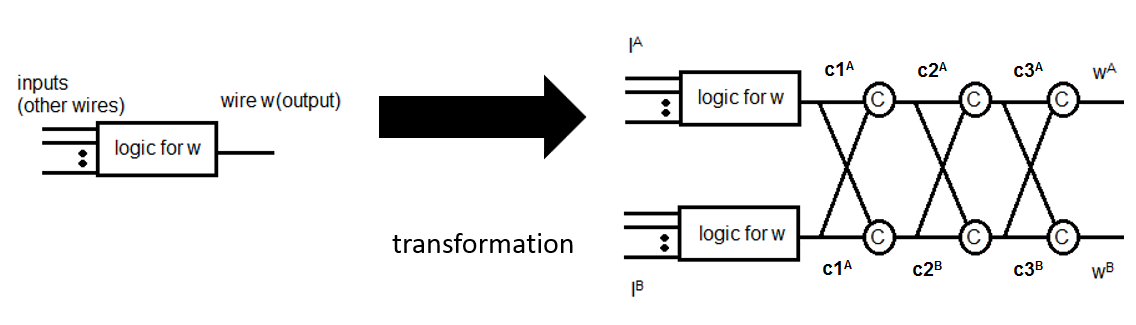
\includegraphics[width=\textwidth]{circuitforproof3}
  \caption{Fault-tolerant transformation: duplicate the original logic for each output wire and adding 3 layers of C-elements}
  \label{fig:dupscheme}
\end{figure}

We want to show that a half circuit from the fault-tolerant circuit has correct function.  To do this, we define a correspondence between states of the original circuit and states of the fault-tolerant circuit.  As a result of the circuit transformation, a state of the fault-tolerant circuit has bits for 8 times as many wires as a state in the original circuit.  Half of those bits are obviously from the A half and half are from the B half of the circuit.  The trace of a fault-tolerant circuit is defined on this combined set of wires.  We first  define the half-circuit mapping $h^B$ for the A half, the half-circuit mapping $h^B$ is similarly defined for the B half.  The half-circuit mapping $h^A: s^{\textit{full}} \to s^A$ where $s^{\textit{full}}$ is the combined state of a fault-tolerant circuit and $s^A$ consists of wires $w^A$ that correspond to the original wires $w$ in the original duplication procedure.  The added wires such as $c1^A$, $c2^A$, $c3^A$ from the duplication procedure is hidden by $h^A$.  We can extend $h^A$ to traces by using the following two steps: first, $h^A$ is applied individually to each state in a trace $\sigma$.  %not sure if I want the mapping to be from variable to variable or specific state to state
%For a trace in the fault-tolerant circuit we project the full states onto a shortened list of wires (ie the wires corresponding to the original circuit). 
The resulting trace may have successive repeated states.  So next we delete all but one of the neighboring repeats, to obtain a valid trace on the shortened list of wires.  Theorem 1 in the upcoming section shows that $h^A(\sigma)$ will be a trace from the original circuit.  
Using this mapping we will show that the original circuit is equivalent to half of the fault-tolerant circuit in both the absence and presence of a single transient fault.
%do I need to define all the new transitions in duplicated circuit?  maybe
\\

%[Why is this the best we can do?]
We compare each half circuit because it is not easy to synchronize and compare the signals between both halves, especially if we reuse the logic blocks from the original circuit.  A simple idea we tried was to insert another C-element before the input is fed into the logic, to synchronize the wires on both halves.  The problem with that is in the original circuit, a wire value change propagates to all inputs at the same time.  Adding another layer of C-elements creates delays at the input to logic blocks and the isochronic fork assumption is violated.  Thus the resulting circuit will not function according to the desired specifications.  (an example can be provided but not sure if needed?)\\  
\begin{figure}
  \centering
    \includegraphics[width=.8\textwidth]{counterexhalf}
  \caption{State graph example to show how b can transition before a or c finishes in both halves in the fault-tolerant circuit}
  \label{fig:counterexhalf}
\end{figure}

Next we examine the traces of each half circuit.  Assume that for the original circuit starting in state 0, both (state 0, state 1, state 3, state 6) and (state 0, state 2, state 5, state 6) are prefixes of valid traces.  Then both halves in the fault-tolerant circuit will transition based on the traces of the original circuit, with the added caveat that for a wire to transition at some state, it must be excited in both halves.  Since only one wire transitions at a time, it is possible for say $a^A$ to transition first and $a^B$ to transition later.  Starting in {\em state 0}, it is possible for the A-half to transition to {\em state 1} ($a^A$ transitions) and for the B-half to transition to {\em state 2} ($c^B$ transitions).  We assume that $a^B$ and $c^A$ do not complete their transitions yet.  Immediately in the A-half, $b^A$ is excited, and in the B-half, $b^B$ is excited.  Since $b$ is excited in both halves, wires $b^A$ and $b^B$ can transition.  That is, the A-half transitions to {\em state 3} and the B-half transitions to {\em state 5}.  And finally, the excited $a^B$ and $c^A$ transitions so that both halves are in {\em state 6}.  The trace so far for the A-half is (state 0, state 1, state 3, state 6) while for the B-half it is (state 0, state 2, state 5, state 6).  Thus the two halves need not have the same trace.  One criticism may be that the current fault-tolerant transformation synchronizes at the outputs of the logic blocks.  If we want to reuse the same logic blocks but synchronize the signals earlier, such as replacing the final C-element in a standard C implementation with a 4C-element, the issue of different traces in the two halves will still occur.  We have already shown earlier that synchronizing the input signals while keeping the original logic block can also result in error.  This points to looking at properties of each half circuit as the right thing to do.\\ 

Another wrong approach for the fault-tolerant transformation is that if we take the following view for transitions, a transition of wire $w$ in the original circuit is complete if both $w^A$ and $w^B$ transitions in the fault-tolerant circuit, then some signals may transition out of order.  We use the earlier example of figure \ref{fig:counterexhalf} to show this as well.  Following the same transitions outlined above, $b^A$ and $b^B$ can finish their transitions before $a^B$ and $c^A$ transitions.  Then the $b+$ transition is actually completed before $a+$ or $c+$ and the combined trace no longer maps back to a valid trace in the original state graph.  Another approach we may take is to record the first transition of a wire in either half of the fault-tolerant circuit.  For example, if $w^A=w^B$ and then $w^A$ transitions, we map this to a transition on $w$ in the original circuit.  This approach ensures the resulting trace is a trace in the original circuit (can be shown by Lemma 1 and Lemma 2.1 in the next section), however, in the presence of faults, it is easy to see that it does not provide any fault tolerance.\\

For the aforementioned reasons, we choose to use the $h^A$ and $h^B$ mappings and compare each half circuit against the original circuit.  Out of the various comparisons methods and circuit transformations that we tried, it is the most reasonable and results in some nice properties.  We will next demonstrate that the half circuits are equivalent to the original circuit in the absence of faults.  Then we show that a similar property is true even when a single fault may occur.

\section{Normal operation analysis}
Now we will discuss the proper wire initializations before going into the Lemmas.  Defining a set of traces of a circuit includes defining the initial state.  For the original circuit, if the circuit starts from this initial state, then the synthesis method ensures semi-modularity in all traces.  However, the proposed fault-tolerant transformation adds logic, and the set of traces and initial state may be different from those of the original circuit, even after applying the half circuit mappings.  Thus we need to ensure that after the transformation, the circuit behaves in a similar way to the original circuit.  That is for an initial state of the fault-tolerant circuit, which is related to the initial state of the original circuit, the resulting traces will behave similarly and have properties such as semi-modularity and the same stopping states as the original circuit. \\

%the half circuits are still semi-modular, has the same transitions as the original circuit and does not stop in non-stopping states of the original circuit. 
%This initial state consistent with semi-modularity also includes the initial values of internal wires.

We show how to define the initial state for the fault-tolerant circuit if given the initial state for the original circuit.  The values for the internal wires must also be set.  These internal wires are initialized to a semi-modularity consistent value.  Given this, we pick the following convenient initializations for the fault-tolerant circuit.  The following procedure covers how to initialize both the wires from the duplication as well as the extra $c1^A$, $c1^B$, $c2^A$, $c2^B$, $c3^A$, $c3^B$ wires that are introduced.
%For all initial states we assume that we know the values of every wire in the circuit, intermediate and visible wires.  The visible wire values are the output wires in the circuit $w$, and the wires $c1$, $c2$ and $c3$'s. The intermediate wires are all other wires, which consists of all the wires within the logic blocks for each output wire.  Given these we will show how to define a corresponding initial state in the duplicated circuit.  %should I delete intermediate?
\begin{definition} A {\em valid initial state} $s'$ for the A-half of the fault-tolerant circuit is constructed from the initial state $s$ of the original circuit.  
For the $w$ logic block and output wire $w$ in the original circuit, the wire values are copied to the corresponding logic block and output wire $w^A$ in the A-half.  The additional wires from the C-element chain are also assigned the same value as $w$.  That is, $s(w)=s'(w^A)=s'(c1^A)=s'(c2^A)=s'(c3^A)$.  This is repeated for all output wires in the original circuit. 
%This completes the construction for the {\em valid initial state} of the A-half circuit.
\end{definition}
%\textbf{
The same construction applies for the B-half circuit as well.  Given this definition, both the A-half and B-half initial states are constructed from the same initial state of the original circuit.  
There is a larger set of states that could serve as initial states of the fault-tolerant circuit, but this definition is sufficient for our purposes.\\

\begin{comment}
%dynamic properties of SM?  I don't think it's needed right now
The input wire values must also satisfy dynamic properties.  Static properties such as the input wire values must be from valid states of the trace is not enough.  The order and the wire transitions also matter.   
The semi-modularity property must be preserved: if the logic block output is excited then it must remain excited until a transition on its output occurs.  Since certain inputs which are valid states and arise from valid transitions may cause the logic block to become unexcited before a transition occurs and thus break the semi-modularity property, we require this more stringent criteria.


In normal operation, the fault-tolerant circuit must have wire values consistent with semi-modular behavior in the original circuit.  
This includes the internal wires which exist in the logic blocks in the original circuit and through duplication also exist in the fault-tolerant circuit.  The actual values of these wires do not matter if the inputs to the logic blocks follow the semi-modularity property, and if the internal wires are initialized properly.
This arises from the original synthesis method to synthesize the circuit from an underlying state graph.  
Additionally, it does not suffice for the inputs to the logic blocks to be from a valid trace of the state graph; the timing matters as well.  The semi-modularity property must be preserved: if the logic block output is excited then it must remain excited until a transition on its output occurs.  Since certain inputs which are valid states and arise from valid transitions may cause the logic block to become unexcited before a transition occurs and thus break the semi-modularity property, we require this more stringent criteria.  %maybe needs an example
Thus to satisfy semi-modularity, the inputs wait at certain input states until the output transitions.  Then the internal wires of the logic block are termed {\em semi-modularity consistent} if the following properties are true:  if the inputs follow semi-modularity then there are no glitches at the output; and once the output is excited it remains excited until the output transitions. \\%newly added
\end{comment}

%To avoid overly clunky sentences, we will assume that fault-tolerant circuits start from the same valid intial state in both halves.  One exception to this assumption is Lemma 1 where only one half circuit is needed to start from a valid initial state since the property is true regardless of the wire values of the other half.\\ 
%For all subsequent discussion in this document, when we talk about the trace of a fault-tolerant circuit we assume that both half circuits start from the same valid initial state.  I will not include this assumption in the following lemma definitions to avoid complicated wording.  %}  
%The one exception is for Lemma 1 where we only require one half circuit to start from a valid initial state.  \\

To prove claims about the fault tolerance of this circuit, we first prove that the circuit behaves similarly to the original circuit under normal operation.  That is, the set of traces of the fault-tolerant circuit after applying a mapping of $h^A$ is equivalent to that of the original circuit.  And likewise after applying a mapping of $h^B$ to the fault-tolerant circuit.  We show this through several Lemmas. Lemma 1 shows for each fault-free half of a circuit, if a transition occurs, it must be a transition in the set of traces of the
%since it's a transition, then all previous transitions must also be in the set of traces, in fact they must all be a sequence of at least one trace (true because if excited, must be excited in all states of same name)
 original circuit.  This is a strong result; it is true for  {\em arbitrary behavior} of
wires in the other half circuit, so long as those wire values are well-formed Boolean values and also does not cause the fault-free half to deviate from well-formed Boolean values.  
This result is also significant later in proving fault tolerance under a single transient fault since at least one of the halves is always fault-free.  %as long as it does not violate digital abstraction
%One additional assumption that we make about the gates and wire values (including in the presence of faults) for Lemma 1 to hold is that wire values are strictly 0 or 1, and transitions from excited gates also only produce 0 or 1 and no in between values, no matter the duration of signals from the input wires.
\\

Note that Lemma 1 allows for the possiblity of the fault-tolerant circuit to stop at states that are not stopping states in the original circuit.  This is an important point as we do not want our transformed circuit to stop prematurely.  We call such premature stopping states, if they exist, as deadlocked states:
\begin{definition}A {\em deadlocked state} is a stopping state of the fault-tolerant circuit but not a stopping state of the original circuit.\end{definition}
We use {\em deadlock} to mean the existence of such deadlocked states.  
Then, Lemma 2 shows deadlock does not occur during normal operation.  Combining these two Lemmas, we can show that all traces in the fault-tolerant circuit can be mapped to a trace in the original circuit.\\
% and all traces in the original can be mapped to duplicated after h mapping?  <-this is obvious though by setting the A half and B half to both transition according to original trace
%[so no deadlock in normal operation??]


\begin{lemma}[0]
Given two identical logic blocks $f$ and $g$, if the inputs into $f$ and $g$ have the same values then:\\
i)  if the outputs are the same value and $f$ is excited then $g$ is also excited.\\
ii)  if the outputs are the same value and $f$ is unexcited then $g$ is also unexcited.\\
iii)  if the outputs are different values and $f$ is excited then $g$ is unexcited.
\end{lemma}
\begin{proof}
i) \& ii)  Since $f$ and $g$ are identical gates or C-elements then if the inputs and output are the same values, $f$ and $g$ must be both excited or both unexcited. \\

iii)  We prove this by contradiction.  Suppose that inputs to $f$ and $g$ are the same and the outputs are different values and both $f$ and $g$ are excited.  This means that for some circuit element that these input values both cause the element to excite to 1 and 0 at the same time.  This cannot happen in any of the elements that we build our circuit from and is therefore a contradiction.
\end{proof}

%MAPPING PROPERTY?
In the following lemmas and theorems we compare a state $s$ in the fault-tolerant circuit with its mapped state $h^A(s)$ in the original circuit.  Due to the mapping and architecture of the circuits, for any wire block $w$, the inputs to the logic block of $w^A$ in the fault-tolerant circuit has the same value as the inputs to the logic block of $w$ in the original circuit.  This fact is used extensively in combination with Lemma 0.  The excitation on $w$ in the original circuit can sometimes be deduced from semi-modularity, then by applying Lemma 0 we can also derive the excitation on $w^A$.  \\
%compare with original circuit: logic block with same inputs.....if input cause block to be excited... if output is same too then the state of logic block is identical.  



This leads to the definition and proof of Lemma 1 as follows:

\begin{lemma}[1]
Consider a fault-tolerant circuit that is fault free and its A half begins in a valid initial state.  For every trace $\sigma$ of this circuit, the following two properties hold: %still kind of weird wording
\begin{itemize}
\item P1: The half-circuit mapping of a prefix of $\sigma$, written as $h^{A}(\sigma_n)$, is also a prefix of a trace of the original circuit, regardless of the wire values in the B half.
%\item P2: The logic blocks in the A half are semi-modularity consistent for all states in $\sigma$
\item P2: For all states $s$ in $\sigma$, a wire $w$ in state $h^A(s)$ is excited in the original circuit if and only if exactly one of the following is true in the fault-tolerant circuit: $c1^A$ is excited or $c1^{A}\neq c2^{A}$ or $c2^{A}\neq c3^A$ or $c3^{A}\neq w^A$.  When one of these conditions holds, we say “the wireblock $w^A$ is excited.”  A wire $w$ in state $h^A(s)$ is unexcited in the original circuit if and only if none of the four conditions are true in the fault-tolerant circuit.  (No more than one of the four conditions mentioned may be true regardless if $w$ is excited or unexcited.) 
\end{itemize}
 
%Let $\sigma_n$ be the sequence of the first $n$ states of a trace $\sigma$ of the fault-tolerant circuit (the trace is possibly finite).  


%In the duplicated circuit, for all traces $\{\sigma\}$ that starts from a valid initial state for half of the circuit ${A,B}$, the following is true.  At each state $s_n$ in the trace mapped to $h^{A,B}(s_n)$ in the original circuit, a wire $w$ is excited if and only if exactly one of the following is true: the gate is excited or $x'^{A,B}\neq x^{A,B}$ or $x^{A,B}\neq w^{A,B}$.  (So for a wire that is not excited in the original circuit, neither the gates or the c-element is excited in the duplicated circuit.)
%need to modify to include two layer c-elements

%If the duplicated circuit is in state $s_n$ and the original circuit is in state $h^A(s_n)$, and for all wires $w$ that are excited in this state $f_w(s_n|_I)\neq w$ in original circuit, then $f_w(s_n|_I) \neq x^A$ or $x^A \neq w^A$ in duplicated circuit (exactly one of these is true).  
%In addition, if wire $w$ is not excited in the original circuit $f_w(s_n|_I)=w$, then in the duplicated circuit half $f_w(s_n|_I)=x^A=w^A$.  
\end{lemma}

\begin{proof}
Let $\sigma$ be an arbitrary trace of the fault-tolerant circuit.  We will show by induction on $n$ that Lemma 1 is true for the length $n$ prefix of the trace $\sigma_n$.  
%We will show by induction on $n$ that for any prefix of the trace $\sigma_n$, where $n$ is an integer from 1 to the length of the trace, $h^A(\sigma_n)$ is a prefix of a trace of the original circuit.
% true but needs to find a new home -> either $h^A(s_n)=h^A(s_{n+1})$ or $T(h^A(s_n), h^A(s_{n+1}))$
We first show the induction hypothesis holds in the base case of $\sigma_1$ consisting of state $s_1$, a valid initial state by construction.
\begin{itemize}
\item State $s_1$ is a valid initial state so $h^A(s_1)$ is a state in the original circuit by construction. %how to compare with OG circuit NEED TO FIX!!
 Thus $h^A(s_1)$ is a prefix of length 1 of a trace in the original circuit and satisfies P1.
%\item We assigned the initial wire values so that the logic blocks are in a semi-modularity consistent state so P2 holds.
\item 
For each wireblock, the valid initial state initializes wires $c1^A$, $c2^A$, $c3^A$ and $w^A$ to the same value.  Therefore only wire $c1^A$ may be excited.  Since the mapping gives identical inputs then by Lemma 0 i) ii) if wire $w$ is excited in the original circuit, $c1^A$ is also excited in the fault-tolerant circuit.
And if wire $w$ is unexcited in the original circuit, then $c1^A$ is unexcited in the fault-tolerant circuit.  This shows that state $s_1$ satisfies P2.    %is this enough.... that the existing states follow that iff statement?
\end{itemize}

The induction step is to assume that the induction hypothesis is true for all length $k$ prefixes of traces of the fault-tolerant circuit.  We will prove that the induction hypothesis is true for all length $k+1$ prefixes.  %/length $k$ prefix  
%We will prove that the induction hypothesis is also true for all $\sigma_{k+1}$ that exist. 
Let $\sigma_k$ be an arbitrary length $k$ prefix and $s_k$ its $k$-th state.  
To show the induction hypothesis is true for all length $k+1$ prefixes, equivalently we show the hypothesis is true for all possible next states $s_{k+1}$ from the state $s_k$.\\

In fact, the possible next states can be partitioned into transitions from each of the cases in Figure \ref{fig:l1helper}.  To see this, we first note that examining the transitions in only the A-half is sufficient.  Transitions in the B-half can be ignored under the $h^A$ mapping because such transitions do not change wire values in the A-half and the resulting states are deleted by the mapping.  We know by the induction hypothesis that P1 and P2 are true for the current state $s_k$.  In particular, P2 states that all wire blocks in state $s_k$ are in one of the cases in Figure \ref{fig:l1helper}.  Only cases 1-4 have excited gates or C-elements that are capable of a transition.  Thus, to cover all possible transitions, it suffices to examine transitions in an excited wire block from cases 1-4. \\
%(By P2, if a wire block $w$ is excited in state $s_k$, then the corresponding wire $w$ is excited in the original circuit in state $h^A(s_k)$.  To cover all transitions, it suffices to examine transitions in an excited wire block from cases 1-4. ) 

% which by P3 applied to state $s_k$, implies that the corresponding wire is also excited in the original circuit.
%By P3, wires in the fault-tolerant circuit may change only if the wire block is excited, which implies wire $w$ is also excited in the original circuit in state $h^A(s_k)$.
 
%Although we need to examine all excited wire blocks at state $s_k$, since they can only be in one of four states, then it suffices to look at what happens if a wire transitions from each state. 
%  Thus for each excited wire block $w$, %need to define wire block

%P3 states that the wire block must be in a state a-d) of figure \ref{fig:l1helper}.  We consider what happens if a wire transitions from each state. 
%logic gate excited = c1^A excited
%possibly add graph to illustrate this
\begin{figure}
  \centering
    \includegraphics[width=\textwidth]{gatewl2}
  \caption{Different cases of P2 for a wireblock, 1-4 correspond to excited wire in the original circuit and 5 is unexcited.  1) case 1, 2) case 2, 3) case 3, 4) case 4, 5) case 5}
  \label{fig:l1helper}
\end{figure}

We first prove P1 and then P2 for the length $k+1$ prefix.  To show P1 is true for state $s_{k+1}$, we must show that $h^A(s_{k+1})$ is a reachable state and that ($h^A(s_{k})$,$h^A(s_{k+1})$) is a transition in the original circuit.  The proof for P1 relies only on the induction hypothesis being true for state $s_k$ and is as follows: \\

Let the transitioning wire block from state $s_k$ be called $w$.  There are four cases that $w$ can be in.  % A transition occurs on a wire block that is in cases 1-4. 
\begin{itemize}  
\item Cases 1-3 (Figure \ref{fig:l1helper}) are considered together.  
If an excited wire block $w$ is in any of these three cases, there is only one possible transition for each case: the new wire value propagates down the C-element chain.  That is, in state $s_{k+1}$, wire block $w$ is in cases 2-4 respectively.  For all three cases, the transition occurs on an intermediate wire and $h^A(s_{k+1})=h^A(s_{k})$.  This is a repeated state under the half circuit mapping applied to the trace and is deleted.  Thus $h^{A}(\sigma_{k+1})=h^{A}(\sigma_k)$ and $h^{A}(\sigma_{k+1})$ must also be a prefix of a trace of the original circuit. 
\item Case 4 (Figure \ref{fig:l1helper}) has only one possible transition which is on wire $w^A$.  Then under the half circuit mapping, wire $w$ transitions from state $h^A(s_k)$ to state $h^A(s_{k+1})$.  By P2, wire $w$ is also excited in state $h^A(s_k)$ and this is a valid transition (i.e., $T(h^A(s_k), h^A(s_{k+1}))$).  Therefore $h^{A}(\sigma_{k+1})$ is a prefix of a trace of the original circuit. 
\end{itemize}

That concludes the proof for P1.  Next, we show that P2 is true for all possible $s_{k+1}$ by showing that $s_{k+1}$ in the fault-tolerant circuit corresponds to $h^A(s_{k+1})$ in the original circuit with certain properties of the wireblocks preserved.  Again, there are four cases that the transitioning wireblock $w$, can be in.  

\begin{itemize}
\item Cases 1-3 (Figure \ref{fig:l1helper}) are considered together.  As mentioned in the P1 proof, the transition occurs on an intermediate wire and $h^A(s_{k+1})=h^A(s_{k})$.  Since $h^A(s_{k+1})=h^A(s_{k})$, then all wires in the original circuit do not change excitations in the new state $h^A(s_{k+1})$.  Then $w$ in the original circuit remains excited in state $h^A(s_{k+1})$, while wireblock $w$ in the fault tolerant circuit is in one of cases 2-4 in state $s_{k+1}$.  Wireblock $w$ satisfies P2.  All other wireblocks in the fault-tolerant circuit do not change cases in the new state $s_{k+1}$.  
Thus all wireblocks of the fault-tolerant circuit in state $s_{k+1}$ satisfy P2.     

%The transition occurs on an intermediate wire and $h^A(s_{k+1})=h^A(s_{k})$.  The wire $w$, in the original circuit, is then excited in state $h^A(s_{k+1})$ and P3 holds for wire $w$.  For the remaining output wires, P3 holds because again $h^A(s_{k+1})=h^A(s_{k})$, so the excitation of all output wires in the original circuit do not change in state $h^A(s_{k+1})$.  The wire blocks in the fault-tolerant circuit also remain in the same case of Figure \ref{fig:l1helper} in $s_{k+1}$.  Thus P3 holds for all wires in state $s_{k+1}$.  Another consequence of $h^A(s_{k+1})=h^A(s_k)$ is that P1 holds.  And lastly no output wire transitions implies the logic blocks stay in a semi-modularity consistent state so that P2 holds.

%\item The first case is for an excited wire $w$.  In the fault-tolerant circuit, wire $c1^A$ is excited and $c1^A=c2^A=c3^A=w^A$, then $c1^A$ transitions.  Then in $s_{k+1}$, the only changes are that $c1^A$ is no longer excited and $c1^A\neq c2^A$, thus wire $w$ satisfies the third induction hypothesis.  Since the transition occurred on an intermediate wire, the set of excited wires in state $h^A(s_{k+1})$ of the original circuit does not change and for both excited wires $v$ where $v\neq w$ and unexcited wires, the third induction hypothesis carries over from $s_k$ to $s_{k+1}$.  Thus the third induction hypothesis is true for all output wires.  Also since the output wires did not change, then $h^A(s_k)=h^A(s_{k+1})$ satisfying the first induction hypothesis.  The output wires not changing also allow the logic blocks to stay in a semi-modularity consistent state.   The induction hypotheses are true for any transition from this case.  %don't know if this needs to be explained more (and add that the non-excited wires are still non-excited?)
%since the inputs to the gate and the intermediate wires did not transition, then the gate is excited or $y^{A,B}\neq v^{A,B}$.  
%do I need to show that non-excited has nothing excited in duplicated
%$w$ is still excited in $h^A(s_{k+1})$ and in state $s_{k+1}$ only $c1^{A}\neq c2^{A}$ is true.   Therefore in this case the property is true for state $s_{k+1}$
%\item The second case is when the signal propagates down to $c2^A$.  In state $s_k$, $c1^A$ is unexcited, $c1^{A}\neq c2^{A}$ and $c2^A=c3^A=w^A$, then $c2^A$ transitions.  Then in state $s_{k+1}$, the changes are $c1^A=c2^A$ and $c2^{A}\neq c3^{A}$ and thus wire $w$ satisfies the third induction hypothesis.  This is also an intermediate wire transition so by similar reasoning to the first case, all induction properties are true for any transition from this case.   
%\item The third case is similar to the second case and occurs when the signal propagates down to $c3^A$.  In state $s_k$, $c1^A$ is unexcited, $c1^A=c2^A$, $c2^{A}\neq c3^{A}$ and $c3^A=w^A$, then $c3^A$ transitions.  
%Then in state $s_{k+1}$, the changes are $c2^A=c3^A$ and $c3^{A}\neq w^{A}$ and thus wire $w$ satisfies the third induction hypothesis.  This is also an intermediate wire transition so by similar reasoning to the first case, all induction properties are true for any transition from this case.   

\item The last case is when a transition occurs from case 4.  That is, $w^A$ transitions in the fault-tolerant circuit from case 4 of Figure \ref{fig:l1helper}.  %The original circuit transitions to state $h^A(s_{k+1})$ where wire $w$ transitions.
As mentioned in the P1 proof, applying the half circuit mapping results in a corresponding transition of wire $w$ in the original circuit.  
%applying the $h^A$ mapping to state $s_{k+1}$ indicates that $w$ transitions in the original circuit.  
These two transitions can change the excitation state of wireblocks/wires in the fault-tolerant circuit and the original circuit respectively.  By P2, the wireblocks in state $s_k$ are partitioned into five cases (Figure \ref{fig:l1helper}).  We examine the changes to a wireblock in each of the five cases due to the $w^A$ transition.  Note that because wire $w^A$ transitions, wireblock $w$ is a special case of case 4 which we deal with separately.
%Next we show P3 holds by examining $w$/$w^A$'s effects in the other wires/wire blocks.  A change in wire $w$ fans out to other logic blocks which may change their excitations in response.  Thus we partition the output wires in the original circuit into four categories: wires that are excited in the current state and excited in the next state, wires that are excited in the current state and unexcited in the next state, wires that are unexcited in the current state and are newly excited in the next state, and wires that are unexcited in the current state and unexcited in the next state.
%these are the only possibilities in the original... look at what happens to these wires in the FT circuit
\begin{itemize}
\item
For wireblocks in cases 1-4 in state $s_k$ (excluding wireblock $w$), we show that these wireblocks remain in the same case in state $s_{k+1}$.  Let us call such a wireblock $v$.  By P2, wire $v$ of the original circuit is excited in state $h^A(s_{k})$.  Since $h^A(\sigma_{k+1})$ is a prefix of a trace (by P1) in a semi-modular circuit and $v$ does not transition, then $v$ must remain excited in state $h^A(s_{k+1})$.  For P2 to be true in state $s_{k+1}$, we must show that wireblock $v$ in the fault-tolerant circuit remains in cases 1-4.  A transition on $w^A$ can only affect the logic block portion of the wireblock.  \\
Case 1 is straight forward since the inputs and output of $c1^A$ in the fault-tolerant circuit and $v$ in the original circuit are the same values, then by Lemma 0 i) wire $c1^A$ must have the same excitation as $v$, that is, excited.  If $v$ is in case 1 in state $s_k$, then $c1^A$ remains excited in state $s_{k+1}$ with no other transitions in $v$, thus $v$ is in case 1 in state $s_{k+1}$.  \\
In Cases 2-4, the logic block of the fault-tolerant circuit is unexcited while $v$ is still excited in the original circuit.  By semi-modularity, wire $v$ remains excited in state $h^A(s_{k+1})$.  In state $s_{k+1}$ and state $h^A(s_{k+1})$, the inputs to $c1^A$ and $v$ are equal but $c1^A$ and $v$ have different values.  By Lemma 0 iii), since $v$ is excited then $c1^A$ is unexcited.  Thus, if wireblock $v$ is in case 2 (or 3 or 4) in state $s_k$, then $c1^A$ remains unexcited in state $s_{k+1}$ and wireblock $v$ remains in case 2 (or 3 or 4) in state $s_{k+1}$.  
Since $v$ stays excited in the original circuit in state $h^A(s_{k+1})$, any wireblocks in these 4 cases satisfy P2 in state $s_{k+1}$.

%For wires $v$ that are excited in state $h^A(s_k)$ and excited in state $h^A(s_{k+1})$ in the original circuit, the wire block $v$ must be in cases 1-4 of Figure \ref{fig:l1helper} at state $s_k$.  If $w^A$ does not feed into wire block $v$ then wire block $v$ stays in the same case in state $s_{k+1}$.  Furthermore, if wire block $v$ is in case 1, then the inputs and $c1^A$ and $v$ wires match in the fault-tolerant and original circuits, thus $c1^A$ is also excited in state $s_{k+1}$ and wire block $v$ remains in case 1.  If wire block $v$ is in cases 2-4, then $c1^A\neq v$ and we cannot apply the same logic.  The correct reasoning is outlined in Figure \ref{fig:sml1} and described as follows.  
%Since $v$ is excited in state $h^A(s_{k+1})$, then $v$ can transition to a state $h^A(s_{k+2})$.  Now we compare the original circuit in state $h^A(s_{k+2})$ and the fault-tolerant circuit in state $s_{k+1}$.
%  The inputs of $v$ in state $h^A(s_{k+2})$ are equal to the inputs to wireblock $v$ in state $s_{k+1}$ (since $v$ is not its own input) and $c1^A=v$, therefore $c1^A$ must be unexcited in state $s_{k+1}$.  Thus wire block $v$ stays in the same case for cases 2-4.  We have shown for all such wires $v$, the corresponding wire block stays in the same case in the fault-tolerant circuit, so P3 holds for wires of this type.

%by semi-modularity $c1^A$ of $v$ in the A-half circuit will not change its excitation state in $s_{k+1}$ and the rest of the corresponding wires of $v$ stays the same, wires of this type satisfy P3.   %semi-modularity part still needs to be fixed

%\begin{figure}
%  \centering
%    \includegraphics[width=\textwidth]{sml1}
%  \caption{An example of wire block $v$ in case 2.  The figure shows wire block $v$ in the fault-tolerant circuit and wire $v$ in the original circuit in states $s_k$ and $s_{k+1}$.  Each arrow denotes a transition}
%  \label{fig:sml1}
%\end{figure}
\item
Wireblock $w$ is a special case of case 4.  Wire $w$ of the original circuit has just transitioned in state $h^A(s_{k+1})$.  Since $w$, the only wire value that changed, is not an input to itself, $w$ is unexcited in state $h^A(s_{k+1})$.  In the fault-tolerant circuit, $w^A$ just transitioned so the wireblock $w$ is in either case 1 or case 5.  By Lemma 0 ii), since $w$ is unexcited in the original circuit $c1^A$ is also unexcited.  Thus wireblock $w$ in state $s_{k+1}$ is in case 5 while wire $w$ in state $h^A(s_{k+1})$ is unexcited.  Thus P2 holds for wire block $w$ in state $s_{k+1}$.

%By semi-modularity, if a wire is excited in state $h^A(s_{k})$ and does not transition, then it remains excited in state $h^A(s_{k+1})$.  
%Thus, the only wire that is excited in state $h^A(s_{k})$ and unexcited in state $h^A(s_{k+1})$ is the transitioning wire $w$ (since $w$ is not its own input).
%  In state $s_{k+1}$, $w^A$ transitions and since $c1^A=w$, $c1^A$ remains unexcited, so wire block $w$ is in case 5 of Figure \ref{fig:l1helper}.  Thus P3 holds for wire $w$.  
\item
For wireblocks in case 5 in state $s_k$, we show that these wires stay in case 5 or transition to case 1 in state $s_{k+1}$.  Let us call such a wireblock $u$.  By P2, $u$ is unexcited in the original circuit in state $h^A(s_{k})$.  There are two possibilities in the next state: $u$ can be excited or unexcited in state $h^A(s_{k+1})$.  We first note that by the half circuit mapping on $s_{k+1}$, the inputs to $u$ in the original circuit and $c1^A$ of wireblock $u$ in the fault-tolerant circuit have the same values, and also $c1^A=u$.  \\
If $u$ is excited, then by Lemma 0 i) $c1^A$ in the fault-tolerant circuit is also excited in state $s_{k+1}$.  Then wireblock $u$ is in case 1 (Figure \ref{fig:l1helper}) in state $s_{k+1}$.  Thus P2 holds for wires of this type in state $s_{k+1}$.\\
And if $u$ remains unexcited in state $h^A(s_{k+1})$, by Lemma 0 ii) $c1^A$ of wireblock $u$ is unexcited in state $s_{k+1}$.  Then wireblock $u$ stays in case 5 of Figure \ref{fig:l1helper}.  Thus P2 holds for wires of this type.
%$u$ that are unexcited in state $h^A(s_{k})$ and transition to excited in state $h^A(s_{k+1})$, in state $s_{k}$ the wire block $u$ is in case 5 of Figure \ref{fig:l1helper}.  But since wire $u$ in the original circuit is excited in state $h^A(s_{k})$ and $c1^A=u$, then $c1^A$ is also excited in state $s_{k+1}$ and the wire block $u$ is in case 1 of Figure \ref{fig:l1helper}.  Thus P3 holds for wires of this type. 
%\item
%Finally for wires that are unexcited in both $h^A(s_k)$ and $h^A(s_{k+1})$, $c1^A$ is unexcited and the wire block stays in case 5 of Figure \ref{fig:l1helper}.  Thus P3 holds for wires of this type. 
\end{itemize}
We have covered all possible wire cases in the circuit.   
Then P2 is true for any transition from case 4. 
\end{itemize}
So the induction hypothesis holds for all possible $\sigma_{k+1}$ and the induction step is complete. \\
By induction on the length of the trace, the first property shows that $h^{A,B}(\sigma_n)$ is the prefix of a trace from the original circuit for all n.
%do I need to show the opposite?  At every step the previous transitions are possible??  Dunno if true for faults though.... also something about collapsed states can't tell the difference?  Can we just map it to a circuit where everything goes together? <- this needs proving?

%so technically one exception is the original w.... but w sort of counts in newly excited if it is indeed newly excited  
%need to expand on newly excited wires
%do I need to define transitions as it occurs here?

%prove each half separately
\end{proof}
By symmetry this is also true for the B half if we exchange A and B in the statement of Lemma 1.  
Note as described previously, the proof for Lemma 1 does not place any restrictions on the other half of the circuit other than that the digital abstraction is not violated for C-elements with inputs from both halves of the circuit (e.g. does not cause hazards in the C-element output).  Thus this lemma is true regardless of whether there is a fault or not in the other half of the circuit.  It guarantees that if there is a next state it must follow the state transitions of the original circuit, but does not guarantee that there will be a next state.\\  %maybe move this to in front of L1

This leads to the next property that we will show: if both halves of the circuit start at the same valid initial state, the wire blocks of the circuit transition in a completely predictable pattern and thus deadlock does not occur.
To avoid overly clunky sentences, we will assume that fault-tolerant circuits start from the same valid intial state in both halves.  One exception to this assumption is Lemma 1 where only one half circuit is needed to start from a valid initial state since the property is true regardless of the wire values of the other half.

\begin{figure}
  \centering
    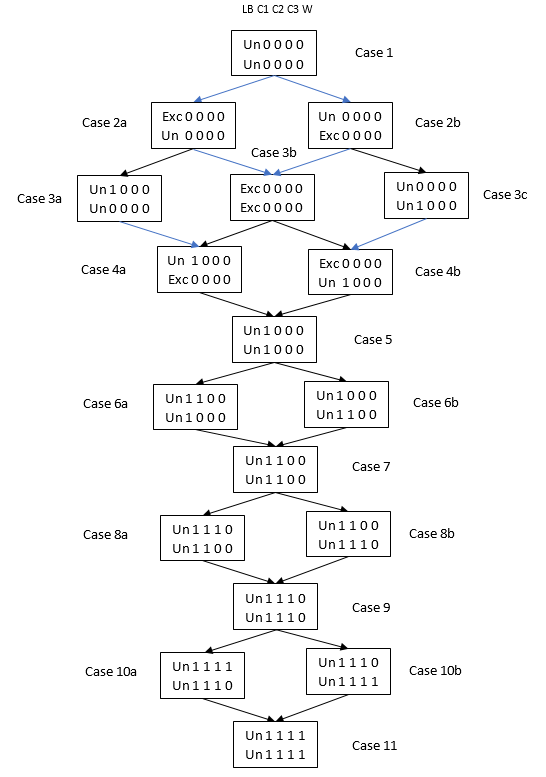
\includegraphics{flowl2c3}
  \caption{The wires in each row are in order of logic block, C1, C2, C3, W.  Each row represents half of the duplicated circuit, ie. top row are A half wires and bottom row are B half wires.  'Un' denotes that the logic block is unexcited and 'Exc' denotes the logic block is excited.  Blue arrows indicate a case change caused by transitions elsewhere in the circuit.  Black arrows indicate a wire transition.}
  \label{fig:l21}
\end{figure}
%fixed 
\begin{lemma}[2.1]
For any trace of the fault-tolerant circuit, each wire block follow the state diagram in Figure \ref{fig:l21} (up to 0 and 1 inversion).
\end{lemma}
\begin{proof}
We show this lemma by induction.  The state diagram in Figure \ref{fig:l21} is incomplete in the sense that after case 11, there are more transitions.  However, case 11 is symmetric to case 1 with only the 0's and 1's inverted and so the transitions from case 11 is also symmetric to the transitions from case 1 with 0's and 1's inverted until it loops back to case 1.  Because of this symmetry, we only need to analyze possible transitions from each case up to case 10.  Also, Lemma 1 applies to both A half and B half which we will use in the body of this proof.\\

We look at the base case of $\sigma_1$ which is also $s_1$ initialized as a valid initial state.  For every wire $w$ in the original circuit, the valid initial state initializes the wires in the fault-tolerant circuit to state a of Figure \ref{fig:l1helper} if wire $w$ is excited, or initializes to state e of Figure \ref{fig:l1helper} if wire $w$ is unexcited.  Because the initialization is the same for both halves, then if $w$ is excited then the logic blocks in the fault-tolerant circuit are in case 3b of Figure \ref{fig:l21} and if $w$ is unexcited then the logic blocks are in case 1 of Figure \ref{fig:l21}.  Thus the lemma property holds for the base case. \\
%is this the pick a trace thing again? (instead of for all traces of length n)

In the induction step, assume that the induction hypothesis is true for trace $\sigma_k$ and we show that it is true for $\sigma_{k+1}$ by looking at state $s_k$.  \\

In state $s_k$, all wire blocks are in a case in the state diagram from the induction hypothesis.  It is easy to see that the only possible wire transitions in state $s_k$ are the transitions (black arrows) in the state diagram.  
%In addition, if $w$ is the transitioning wire block then because $w$ does not feedback to itself and the input wires do not transition, the logic blocks do not change excitations (other than when $c1$ transitions).  Thus the black arrows show the only possible transitions in the state diagram from state $s_k$.  
For each transition, we must verify that all wire blocks in the new state $s_{k+1}$ either remain in the same case or transition according to the state diagram in Figure \ref{fig:l21}.  Thus we need to investigate the changes in the wire block that transitions as well as the transition's effects on all other wire blocks. 
%For all possible transitions from $s_k$, we must verify that wire blocks in the new state $s_{k+1}$ either remain in the same case or transition according to the state diagram in Figure \ref{fig:l21}.  It is easy to see that the transitions (black arrows) in the figure are the only possible wire transitions when the wire blocks are in a case in the state diagram.  Thus we need to investigate the state changes when a wire block transitions as well as the transition's effects on all other wire blocks. 

%It is clear that transitions and logic block changes in the state diagram can occur.  Furthermore, we can easily verify that the wires in the C-element chains ($c1$, $c2$, $c3$, $w$) behave as the arrows indicate with no additional possibilities.  Thus we need to show that no additional changes in the logic blocks can occur.  
%Because the arrows do not always indicate wire transitions (some are changes in excitation of the logic blocks which are in response to transitions of other output wires), we need only to verify for the transitions that do occur (black arrows), that they do not cause the other logic blocks (and itself) to behave inappropriately.
\begin{itemize}
%\item
%Case 1:  Nothing within the wire block can transition.  It is waiting for its input wires to change.  Once a logic block is excited it changes to case 2a or 2b. %this transition needs not occur, 
\item
Cases $2a\rightarrow 3a$, $2b\rightarrow 3c$, $3b\rightarrow 4a$, $3b\rightarrow 4b$, $4a\rightarrow 5$, $4b\rightarrow 5$, $5\rightarrow 6a$, $5\rightarrow 6b$, $6a\rightarrow 7$, $6b\rightarrow 7$, $7\rightarrow 8a$, $7\rightarrow 8b$, $8a\rightarrow 9$, $8b\rightarrow 9$: \\ 
Let the transition be on wire block $w$.  The transition is on an intermediate wire so the logic blocks of $w$ do not change excitations other than when $c1$ transitions.  
For the same reason, the transition does not affect the excitations in logic blocks of wire blocks other than $w$, thus those wire blocks stay in the same state in $s_{k+1}$.  
%In case 2a, when $c1^A$ transitions, 
%It is also possible that the unexcited logic block becomes excited and go to case 3b at the next state.  However the excited logic block cannot become unexcited (without the corresponding $c1$ transition) due to semi-modularity and Lemma 1.  Case 2b is similar.
%\item
%Case 3a/3b/3c:  In case 3a, it is possible for the logic block in B-half to become excited, and change to 4a.  The logic block in A-half cannot be excited again while $c1^A=1$ because that violates Lemma 1.  Case 3c is similar to 3a.  From case 3b, when $c1^A$ or $c1^B$ transitions, the next state is 4a or 4b.  The excited logic blocks cannot become unexcited due to semi-modularity and Lemma 1.
%\item
%Case 4a/4b:
%In case 4a, the logic block in B-half is excited and can transition to case 5.  The excited logic block cannot become unexcited due to semi-modularity and Lemma 1.  The already transitioned logic block (unexcited) cannot be excited again due to same reasoning as the above cases (Lemma 1).  Case 4b is similar.
%\item
%Case 3a/3b:   If a transition occurs in these cases for wire block $w$, the only excited wires are $c1^{B}$ or $c1^{A}$ respectively.  By the same argument as case 2, the excitation state of the 4C-element for all wires in $s_{n+1}$ must remain the same (other than the one that transitions).  Thus in $s_{n+1}$ wire block $w$ is in case 4 while all other wire blocks remains in the same case from $s_n$ and thus all wire blocks are in a case in the figure. \\
%Cases 5/6a/6b/7/8a/8b:  In these cases for wire block $w$, the only wires able to transition are the excited C-element wires and transitions according to the state graph in figure \ref{fig:l21}.  The only possible additional transitions would come from the logic block but we know that the already transitioned logic block cannot be excited again by Lemma 1.
\item
Cases $9\rightarrow10a$, $9\rightarrow10b$, $10a\rightarrow11$, $10b\rightarrow11$:  \\
Again let the transition be in wire block $w$.  The transition is on an output wire which can change logic block excitations.  We first show that the logic blocks are not excited in wire block $w$ itself after the transition.  This is immediate because $w$ does not feedback to itself and the input wires do not change their values.  It is also true that only wire blocks that $w^A$ and $w^B$ feed into, can change logic block excitations due to the transitions in $w^A$ and $w^B$.  
Next, we examine the effects of the transitions on wire blocks $v$ where $w$ feeds into $v$ and $v$ may be in any cases of Figure \ref{fig:l21}.  
%The above discussions showed that if a wire block is in cases 1-8a/8b, then their logic blocks cannot change excitation other than indicated by the state diagram.  A similar reasoning can be applied to case 9.  By Lemma 1, if any wire blocks are in case 9 and the transition is not in this wire block, then its logic blocks cannot change excitations.  Wire blocks in cases 10a/10b are tricky because we must use a different technique to show that the logic blocks cannot be excited because half of the circuit has completed its transitions.  %Wire blocks in cases 10a/10b are tricky because we cannot directly apply Lemma 1 on the half that has completed its transition to show that its logic block cannot be excited.  
%In cases 1-8a/8b, all transitions happen on intermediate wires so the other wires blocks stay in their previous states.  
\begin{itemize}
\item
If $v$ is in cases $1,2a,2b,\dots9$, the wire blocks can be summarized into three: each half has either an excited logic block and excited wire block, unexcited logic block and excited wire block, or unexcited logic block and unexcited wire block.  For excited logic block and excited wire block (e.g., A-half in case 2a), the new transition cannot cause the excited logic block to become unexcited as it would violate semi-modularity in the original circuit.  For unexcited logic block and excited wire block (e.g., A-half in case 4a), the transition also cannot excite the logic block as it would violate P3 in Lemma 1.  It is possible for unexcited logic blocks with unexcited wire blocks to become excited (e.g., both A and B-half in case 1); all such case changes are covered by the blue arrows.  Thus we have shown that for $v$ in cases 1-8a/8b, changes in $v$ caused by a transition in $w$ follow the state diagram.  
%Thus we need to show that when an output/input wire transitions in cases 9/10a/10b, the transition does not change excitations in logic blocks of all wires in cases 10a/10b. \\  
\item
Next we show that a transition in $w$ does not change excitations in logic blocks of all wires $v$ in cases 10a or 10b.  This is shown by contradiction.  
First we assume that wire block $v$ is in case 10a, and that the $w^A$ transition excites the A-half of the logic block of $v$ in state $s_{k+1}$.  The $w^B$ transition can be ignored because the logic block in the B-half of $v$ cannot be excited as it would violate P3 in Lemma 1.  In state $s_k$, an output wire mismatch is possible only if the wire blocks are in cases 10a or 10b.  Thus for all mismatched wires $u$ in state $s_k$, $c3^A=c3^B$ (${u}$ includes $v$).  Wire $w^A$ transitioning does not change the values of those wires so in state $s_{k+1}$, wires $u$ stay mismatched and their $c3^A=c3^B$.  In state $s_{k+1}$, there is one newly mismatched wire, $w$, which also has $c3^A=c3^B$.  In other words all mismatched wires in $s_{k+1}$ have an output wire that is excited. Then from $s_{k+1}$, we show there is a reachable state that contradicts the initial assumptions.  We choose a sequence of transitions such that all mismatched wires except $v$ become equal.  No other transitions occur.  In that later state, the excited A-half logic block of $v$ is still excited due to semi-modularity in the original circuit.  %semi-modularity... also why is A-half excited?  Also SM
Since the input wires on both halves of wire block $v$ are equal and $c1^A=c1^B$, then the B-half logic block must be excited too.  The state for the B-half violates P3 of Lemma 1 and a contradiction is found. %may need a picture
 Therefore, a wire transition in $w^A$ or $w^B$ cannot excite the logic blocks of a wire in case 10a.  Wires in case 10b are similar.
\end{itemize}
%Lastly we also show that the logic blocks are not excited in wire block $w$ itself after the transition.  This is immediate because $w$ does not feedback to itself and the input wires do not change their values.  \\
Therefore the transitions in this case allow all wire blocks of the circuit to follow the state diagram in Figure \ref{fig:l21}.\\

%We assume that the output wires cannot directly feed back into its logic block so that 10a or 10b cannot cause its own logic block to be excited.  For other logic blocks in case 10a or 10b, a transition in $w^A$ or $w^B$ cannot change the excitation in the other logic blocks.  This is shown by contradiction.  
%Assume that there exists another logic block in case 10a and that the $w^A$ transition causes an excitation of wire $v$ in state $s_{k+1}$ (10a and 10b are symmetric so we only have to show for one of them).  In state $s_k$ an output wire mismatch is possible only if it is in cases 10a or 10b.  Thus for all wires $u$ where $u^A\neq u^B$, $c2^A=c2^B$ (which includes $v$).  $w^A$ transitioning does not change the values of those wires so the property is true in state $s_{k+1}$ as well.  It is also true of the newly mismatched wire $w$.  In other words all mismatched wires in $s_{k+1}$ have an output wire that is excited. Then from $s_{k+1}$ there exists a sequence of transitions of the mismatched wires so that they become equal in a later state (other than wire $v$).  In that later state, the excited logic block of $v$ must still be excited due to semi-modularity.  Since the input wires on both halves are equal, the logic block in the other half must be excited while its output wire is excited too.  This violates Lemma 1 and produces a contradiction.  Therefore a transition to 10a or 10b cannot excite the logic blocks in case 10a or 10b in other wire blocks.\\
%From case 10a or 10b, there may be a transition to case 11 with a corresponding change in the output wires.  Again this cannot excite logic blocks of wires in case 10a or 10b by repeating the argument above in letting the circuit transition until there are no mismatched wires which contradicts Lemma 1.

%still a slight problem here
\end{itemize}
This shows that all wire blocks in all possible $s_{k+1}$ follow the state diagram, and the induction step is complete.\\
By induction on the consecutive states of the trace, the above argument shows that all wire blocks of a fault-tolerant circuit follow the state diagram in Figure \ref{fig:l21} for all traces. \\
\end{proof}
%may be that I don't need how all the intermediate wires go... but just need the at most one of input excitation and outputs can be mismatched.  But this needs to include if outputs are mismatched then the C-element is the same.... which I think I need to show the signals propagating through??
It is now easy to show that deadlock does not occur since each wire block must be in one of the configurations of figure \ref{fig:l21}.
\begin{lemma}[2.2]
For all traces $\sigma$ in the fault-tolerant circuit, deadlock does not occur.
\end{lemma}
\begin{proof}
To show that deadlock does not occur, we show that we can always find an excited wire at any state $s_k$ in a trace of the fault-tolerant circuit.  The state $s_k$ can be split into two cases, one is that all output wire pairs in the A half and B half are equal, the second is that there exists at least one wire $v$ such that $v^A\neq v^B$.  In the first case, if every output wire pair are equal, then $h^A(s_n)=h^B(s_n)$ and there exists an excited wire $u$ in the original circuit.  By Lemma 1 both halves of the duplicated circuit for $u$ is excited.  By Lemma 2.1, the circuit must be in case 2-6 for $u$.  In each of these cases at least one wire is excited.  \\
In the second case, for some wire $v$ such that $v^A\neq v^B$, then using Lemma 2.1 wire block $v$ is in case 7a or 7b which has an excited wire, either $v^A$ or $v^B$.  Since there are next transitions for both cases, deadlock does not occur.
\end{proof}

Combining the results of the previous Lemmas shows that the fault-tolerant circuit is equivalent to the original circuit under normal operation.  This is defined formally in a theorem as follows:
\begin{theorem}[1]
For all traces $\sigma$ in the fault-tolerant circuit, $h^{A}(\sigma_n)$ or $h^{B}(\sigma_n)$ is a prefix of a trace in the original circuit for all $n \in \mathbb{N}$.  (h might make the trace shorter, so the prefix will not be of length n) %what was the point of the deadlock thing?
\end{theorem}
\begin{proof}
Apply Lemma 1 then $h^{A}(\sigma_n)$ or $h^{B}(\sigma_n)$ is a prefix of a trace.  From Lemma 2.2, no deadlock occurs so it is true for all $n\in \mathbb{N}$.
\end{proof}
%with these 3 properties show the original claim
\section{Single transient fault analysis}
%fix this
Next we consider what happens to the fault-tolerant circuit under a single transient fault.  A {\em transient fault} on a wire $w$ causes a transition i.e. flips the bit of $w$.  After the transient event, the affected wire transitions based on its inputs.  %do I need to talk about when transient is not ~x?  ie hold same value?  That's the same as a longer delay
\begin{figure}
  \centering
    \includegraphics[width=\textwidth]{faultexes}
  \caption{Effects of a transient fault.  The left most figure is the state right before a transient fault occurs.  The transition due to the transient fault is denoted by the red F and arrow.   \\
  a) An AND gate, the transient fault causes a transition in $w$ to 0 but the inputs resurrect it back to 1 sometime later.   \\
  b) An AND gate that is excited before the transient fault.  The transient fault causes a transition that would happen anyway, $w$ stays at the correct value 1 after the transition.\\
  c) A C-element.  Its inputs are mismatched so the gate is in a hold state.  When the transient fault causes a transition to 0, the faulty 0 value may persist.
  }
  \label{fig:faultx}
\end{figure}
Examples of the transient fault occuring to gates in different states are shown in Figure \ref{fig:faultx}.  Depending on the inputs and the specific gate, the transient fault can cause a transition to a faulty value and transition back to the previous value; or it can cause a transition that would happen anyway and thus do not affect the gate/ circuit; or the faulty value may be stored in memory elements like the C-element in the hold state.

%new 4/30
We also want to define a faulty trace, which is the trace of a circuit that has a single transient fault.  Formally, the definition is as follows:
\begin{definition}
A {\em faulty trace} is a trace of the circuit where for all $k$, a transition from $s_k$ to $s_{k+1}$ is either a transition as defined in the fault-free case, or a transition through a transient fault.
%there exists an $n$ where $\sigma_n$ is a prefix of a trace of the fault free circuit, then the $n+1$st transition is a transient fault.  After the fault occurs, the circuit continues to transition .
\end{definition}
Transitions after the fault is based on circuit rules and not necessarily the state graph.  To see this, note that the state graph does not necessarily include all possible states of the circuit.  The circuit synthesis technique is designed such that if the circuit is in a state of the state graph, the circuit follows the state graph.  However, a fault may cause $s_{n+1}$ to be in a previously unreachable state.  Then the transitions are governed by the circuit rules of the gates that make up the circuit.\\ %end new

It is useful to extend the concept of excited wireblocks to include wireblocks from faulty traces.  Since we assume the fault is in the B-half, the A-half is fault-free and by Lemma 1, the wireblock in one of cases 1-5 of Figure \ref{fig:l1helper}.  
\begin{definition}
An {\em excited wireblock} is any wireblock that is in cases 1-4 of Figure \ref{fig:l1helper}.  
\end{definition}
Also by Lemma 1, a wireblock is excited if and only if the corresponding wire in the original circuit is also excited.\\

The next major theorem states that a faulty trace in the fault-tolerant circuit maps to a fair trace in the original circuit. To prove this, we need to show that if a wire $w$ in the original circuit is excited, it will eventually transition.  Equivalently, if a wireblock $w$ in the fault-tolerant circuit is excited, it will eventually transition. We assume that the fault happens only in the B-half and in some wireblock $v$. By semi-modularity, the excited A-half of the wireblock remains excited until its output transitions. The transition is guaranteed to happen only if the B-half logic block is permanently excited too, and to the same value as the A-half.\\

The transient fault can be split into two cases: the fault occurs on the $c2^B$ or $c3^B$ wires of $v$, or the fault occurs on the remaining wires $c1^B$ or $v^B$. For the first case, if the fault occurs on the $c2^B$ or $c3^B$ wires, we can directly show that if a wireblock is excited, then it will eventually transition. The result is shown in Lemma 3. However, if the fault occurs on $c1^B$ or $v^B$, the reasoning is more complex. The result is shown in Lemma 4 and 5.\\



We also use the following lemma from Beerel \& Meng (1991).
\begin{lemma}[3.2]Given a live semi-modular speed-independent asynchronous control circuit, all cycles of states in the valid ESG (fault-free traces) must contain all signal (wire) transitions.\\
\end{lemma}
%The next major theorem states that a faulty trace in the fault-tolerant circuit maps to a fair trace in the original circuit. To prove this, we need to show that if a wireblock in the fault-tolerant circuit is excited, it will eventually transition. We assume the fault happens only in the B-half and in some wireblock $v$. By semi-modularity, the excited A-half of the wireblock remains excited until its output transitions. The transition is guaranteed to happen only if the B-half logic block is permanently excited too, and to the same value as the A-half.\\
%
%We first take note of some properties of semi-modular and fault-tolerant circuits. \\
%
%Lemma 3.2 from Beerel \& Meng states that all cycles of states in live semi-modular circuits must contain all signal transitions.\\
%
%Thus, if the theorem that we want to prove is false, then there exists some excited wireblock that does not transition. B\&M's lemma implies that after the mapping, the original circuit stops in some state. This also implies that the A-half of the fault-tolerant circuit also stops. Assuming the A-half stops, we prove that the output pairs eventually have the same value, that is, $w^A=w^B$ for each wireblock $w$. This is split into two cases, when the fault occurs on the $c2^B$ or $c3^B$ wires of $v$, and when the fault occurs on the remaining wires $c1^B$ or $v^B$. 
%end first attempt

%Lemma 3 shows that if the A-half stops and the single fault occurs on the $c2^B$ or $c3^B$ wires of $v$, . 

%Next we show that if a single transient fault occurs on any wire, the fault free half circuit will be equivalent to the original circuit in some sense. Suppose a fault happens in the B-half, according to Lemma 1, the A-half can never be in a state inconsistent to the original circuit. But we have not proved that the A-half does not stop prematurely compared to the original circuit. Towards this goal, we prove two lemmas: Lemma 3 shows if a single fault occurs on the $c2$ or $c3$ wires of some wire $w$, the output wires still follow the original state graph. Lemma 4 shows if a fault occurs on any of the other wires, then the $c2$ or $c3$ wires follow a similar state graph as the non-fault case and thus the output wire pairs can never be different at deadlock. Then these lemmas combine to show that there is no deadlock. A complete trace is defined similarly for the fault-tolerant circuit. That is, the trace after mapping must be a complete trace in the original circuit. The completeness property must be treated separately because there are two halves in the fault-tolerant circuit and one side needs the other to transition. Thus, we need to show that even in the presence of a transient fault, each wireblock will eventually transition. 

%To do this we prove some properties that are true when a single transient fault occurs on a wire. We partition the wires into two sets based on their properties when a single transient fault is added. Lemma 3 shows that if a single fault occurs on the $c2$ or $c3$ wires for some wire $w$, the output wires still follow the original state graph. Lemma 4 shows that if a fault occurs to any of the other wires, then the $c2$ or $c3$ wires follow a similar order to the non-fault case and thus the output wire pairs can never be different at deadlock. Then we combine these Lemmas to show that there is no deadlock.

\begin{lemma}[3]
For any faulty trace $\sigma$ in the fault-tolerant circuit, if the transient fault occurs on wires $c2^B$ or $c3^B$ of some wireblock $v$, then if $w$ is an excited wireblock, $w^A$ will transition.

%For any faulty trace $\sigma$ in the fault-tolerant circuit where the A-half stops, if the transient fault occurs on wires $c2^B$ or $c3^B$ of some wire block $v$, then the circuit stops and for each wireblock $w$, wire values $w^A=w^B$.
\end{lemma}
%need major rewording maybe after defining faulty trace
\begin{figure}
\centering
\includegraphics{L3helperfull}
\caption{The projection of the states in figure \ref{fig:l21} from Lemma 2.1 onto the wires $c1^A$, $c1^B$ and $w^A$, $w^B$. This forms the input and output characteristic of a wire block of a fault-free trace.}
\label{fig:l3helper}
\end{figure}

\begin{proof}
We use NuSMV to prove this. For each wireblock $w$, by Lemma 2.1, the pair of inputs ($c1^A$, $c1^B$) and outputs ($w^A$, $w^B$) of a fault-free trace follow the state diagram shown in Figure \ref{fig:l3helper}. We can view the circuit as composed of two components, the faulty wireblock $v$ and the rest of the circuit. The faulty wireblock $v$ takes inputs from the rest of the circuit and has logic blocks that converts the inputs into wire values $c1^A$ and $c1^B$. Wireblock $v$ produces outputs $v^A$ and $v^B$, which the rest of the circuit takes as inputs. Thus, if we can prove that the outputs $v^A$ and $v^B$ follow the state diagram, then the rest of the circuit cannot tell the difference between this faulty trace and a fault-free trace. \\

The strategy of the proof focuses on interactions between wireblock $v$ and the rest of the circuit. Assume $c1^A$ and $c1^B$ transition as in the fault-free trace, then if $v^A$ and $v^B$ follow the state diagram (Figure \ref{fig:l3helper}), this validates our assumptions for $c1^A$ and $c1^B$ and at the same time shows $v^A$ and $v^B$ follow the state diagram. \\

Wires $c1^A$ and $c1^B$ of a fault-free trace transition as follows: Lemma 3.2 (Beerel \& Meng) states that wires $c1^A$ and $c1^B$ become excited and transition an infinite number of times. In NuSMV, we model $c1^A$ and $c1^B$ as being excited infinitely often and excited only after the previous $v^A$ and $v^B$ transitions complete. We also model the rest of wireblock $v$, that is, the $c2^A$, $c2^B$, $c3^A$, $c3^B$, $v^A$ and $v^B$ wires. A transient fault occurs on wires $c2^B$ or $c3^B$ anytime during the trace. The specifications that are checked using NuSMV are that $v^A$ and $v^B$ transition according to the state diagram (Figure \ref{fig:l3helper}). \\

Running the NuSMV model show that these properties are indeed true. Then for wireblock $v$, once it is excited $v^A$ will transition. For all other wireblocks $u$, since they don't have faults then Lemma 2.1 apply and if $u$ is excited, $u^A$ will transition. 
%We use NuSMV to verify that if a transient fault occurs on wire $c2^B$ or $c3^B$ of wire block $w$, the input-output characteristic of the local C-element chain does not change. Under normal operation, by Lemma 2.1, the pair of inputs ($c1^A$, $c1^B$) and outputs ($w^A$, $w^B$) follow the state diagram shown in Figure \ref{fig:l3helper}. Thus, the property verified in NuSMV is that when a single transient fault occurs on wires $c2^B$ or $c3^B$, the transitions follow the state diagram in the figure. The fault is masked when this happens. \\
% this is kind of by induction, the inputs from the other parts of the system will be correct as long as the output of $w$ is correct. The error is masked if the input output characteristic is still the same
%We first deal with the $0\to 1 \to 0$ fault on $c2^A$. 

%We go through some examples of a transient fault on $c3^B$ to demonstrate why the resulting trace follows the state diagram. We look at the trace when a transient occurs for $v$ in a state in Figure \ref{fig:l21}
% By Lemma 2.1, the normal circuit is in a state in Figure \ref{fig:l21}, so we observe all possible transient induced traces by placing a transient starting at each state in Figure \ref{fig:l21}.
\end{proof}
%By symmetry this is also true for transients in the A half if we exchange A and B in the statement of Lemma 3.\\

%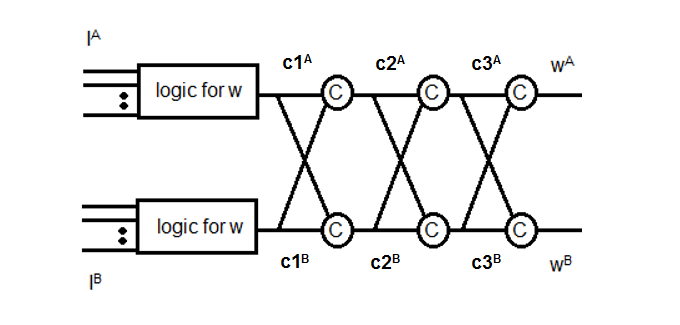
\includegraphics[width=.8\textwidth]{gatew}
\begin{figure}
\centering
\includegraphics{flowl4c3full}
\caption{The wires in each row are in order of $c1$, $c2$ and $c3$. Each row represents half of the duplicated circuit, i.e. top row are A half wires and bottom row are B half wires. Note that case 5 transitions according to case 1 except with the 0's and 1's inverted. The states transition after that are inverted versions of state 2-4 until it transitions back to state 1 (uninverted).}
\label{fig:l4}
\end{figure}

We showed that if a fault occurs on the $c2^B$ or $c3^B$ wires, then if a wireblock is excited, it will eventually transition. 
Next, we show the same result for when the fault occurs on $c1^B$ or $v^B$ wires. 

The transition is guaranteed to happen only if the B-half logic block is permanently excited too, and to the same value as the A-half.

%then the $c2$ or $c3$ wires of each wire block of the circuit transition according to Figure \ref{fig:l4}. The state graph of Figure \ref{fig:l4} is similar to projecting the state graph of Figure \ref{fig:l21} onto the $c1$, $c2$ and $c3$ wires, with the exception that the $c1$ wire value is not known in the faulty half. Despite this, the following lemma is true and we can then conclude that the output wire pairs are never mismatched at deadlock. 


\begin{lemma}[4]
For any faulty trace $\sigma$ in the fault-tolerant circuit, if the transient fault occurs on wires $c1^B$ or $v^B$ of some wireblock $v$, then for each wireblock $u$, at least one of $c2^A=c2^B$ or $c3^A=c3^B$ is true.\end{lemma}
\begin{proof}
We first show that each wireblock $u$ follow the state graph of Figure \ref{fig:l4}. 
We will show by induction on $n$ that this is true for the length $n$ prefix of the trace $\sigma_n$.\\ %how to make it seem like prefix not trace modifies sigma_n

We show the induction hypothesis holds in the base case of $\sigma_1$ consisting of state $s_1$, a valid initial state with no faults. As noted in Lemma 2.1, each wireblock must be in case 1 or case 3b of Figure \ref{fig:l21}. Projecting these wireblocks onto its $c1$, $c2$ and $c3$ wires result in case 1 in Figure \ref{fig:l4}, thus the base case satisfies the induction hypothesis.\\

The induction step is to assume that the induction hypothesis is true for all length $k$ prefixes of traces of the fault-tolerant circuit. 
To show the induction hypothesis is true for all length $k+1$ prefixes, equivalently we show the hypothesis is true for all possible next states $s_{k+1}$ from the state $s_k$. Let the transitioning wireblock from state $s_k$ be called $w$. By the induction hypothesis, $w$ in state $s_k$ may be in any one of the cases in Figure \ref{fig:l4}, so we check for each case that the wire block transitions according to Figure \ref{fig:l4}. We make a further simplification and only analyze when $w$ is in cases 1-5 because transitions from case 6-10 is symmetric to transitions from case 1-5 with 0's and 1's inverted. For example, case 6 is symmetric to case 1 and has the corresponding transition to case 7 as case 1 has to case 2, and so on.\\

%so we observe the effects of the next transition on such a wire block. 
%we then observe how the case may change for that wire block in the next state $s_{k+1}$. 
%For each case that a wire block may be in, we then investigate the case changes in all possible next states $s_{k+1}$. 
The wire value of $c1^B$ is denoted by $X$ in the figure because it is possible that a fault on $c1^B$ or $v^B$ of wireblock $v$ has already occurred in the trace, so the value of wire $c1^B$ of other wireblocks may be affected by that fault. We do not know the value of $X$ except that it is either 0 or 1. Although we don't show the values for $w^B$, we also denote $w^B$ by $X$. Note that this representation also works for the wireblock $v$ when there is a fault on either $c1^B$ or $v^B$ so it encompasses all wireblocks of the circuit.
%(Despite the possibility of a fault, we assume that wire $c1^B$ has value of either 0 or 1 and that even with hazards on $c1^B$, the $c2$ wires transition to either 0 or 1.<-should already be covered) 
Also, we do not consider a $c1^B$ or $w^B$ transition because such a transition is covered by $X$. %X covers both cases when $c1^B$ is 0 or 1.
The possible next transitions from each of the cases is as follows:
%the cases do not depend on the wire value of $c1^B$
%that will result in the wire block staying in the same case.
\begin{itemize}
\item
Case 1: If the transitioning wireblock is in case 1, its $c2$ and $c3$ wires are not excited and only the $c1^A$ and $w^A$ wires may be excited. Therefore, the wireblock either stays in this case or transitions to case 2 in state $s_{k+1}$. %(must prove both the state, and the transition, if there is any... follows the state graph)
\item
Case 2/3a/3b: If the transitioning wireblock is in one of these cases, by Lemma 1, wire $w^A$ must be 0. Also, by Lemma 1, $c1^A$ cannot be excited as it would violate semi-modularity. Thus, the only excited wires are the $c2$ wires. 
Therefore, if the wireblock is in case 2, it transitions to case 3a or 3b in state $s_{k+1}$. And if the wireblock is in case 3a or 3b, it transitions to case 4 in state $s_{k+1}$.
%I might need to show the excited ness of the good logic gate
\item
Cases 4/5a/5b: If the transitioning wireblock is in one of these cases, again, by Lemma 1, wire $w^A$ must be 0. And again, by Lemma 1, wire $c1^A$ cannot be excited as it would violate semi-modularity. Thus, the only excited wires are the $c3$ wires. Therefore, if the wireblock is in case 4, it transitions to case 5a or 5b; and if the wireblock is in case 5a or 5b, it transitions to case 6.
\end{itemize}
Thus, in all possible next states $s_{k+1}$, wireblock $w$ transitions according to Figure \ref{fig:l4}. For all other wireblocks, since they do not transition, they stay in the same cases as in state $s_k$. So, the induction hypothesis holds for all length $k+1$ prefixes of traces and the induction step is complete. 
By induction on the length of the trace, in each trace $\sigma$, each wireblock $u$ transitions according to Figure \ref{fig:l4}. \\ 
For all states in Figure \ref{fig:l4}, at least one of $c2^A=c2^B$ or $c3^A=c3^B$ is true. It follows that for each wireblock $u$, at least one of $c2^A=c2^B$ or $c3^A=c3^B$ is true.
\end{proof}
Lemma 4 shows that at least one of the $c2$ or $c3$ wire pairs have the same values. The next theorem uses this property to show that an excited wireblock will transition when the transient fault is on the $c1^B$ or $v^B$ wires.\\
%all output wire pairs at an assumed deadlock state must be equal, which causes a contradiction, and thus the fault-tolerant circuit does not deadlock under a single transient fault.\\

\begin{lemma}[5]
For any faulty trace $\sigma$ in the fault-tolerant circuit, if the transient fault occurs on wires $c1^B$ or $v^B$ of some wireblock $v$, then if $w$ is an excited wireblock, $w^A$ will transition.
\end{lemma}
\begin{proof}
We prove by contradiction. Suppose that there is some wireblock $w$ in the fault-tolerant circuit that is excited but $w^A$ never transitions. Beerel \& Meng's lemma implies that after the mapping, $w$ doesn't transition in the original circuit and the circuit stops eventually in some state. Thus, the A-half of the fault-tolerant circuit also eventually stops and has no excited wires. By Lemma 4, since at least one of $c2^A=c2^B$ or $c3^A=c3^B$ is true for all wireblocks, then $c3^A=c3^B$ and subsequently $u^A=u^B$ are true for each wireblock $u$ when the A-half stops.  This is illustrated in Figure \ref{fig:t2}.  Furthermore $u^B$ cannot transition again since the A-half is stopped.  Then the inputs to the A-half and B-half of wireblock $w$ have the same values.  By the $h^A()$ mapping, the inputs to the $w$ logic block in the original circuit also have the same values.  By Lemma 0 i), since wire $w$ is excited in the original circuit, then wire $c1^B$ is also excited. Since the inputs to $c1^B$ do not change, $c1^B$ eventually transitions. By similar reasoning, $c1^A$ must have transitioned as well and so $c1^A=c1^B$ which forces $c2^{A,B}$ then $c3^{A,B}$ then $w^{A,B}$ to the new value.  This violates our initial assumption that $w^A$ does not transition.  Thus, for an excited wireblock $w$, $w^A$ will transition. 
\end{proof}

\begin{figure}
\centering
\includegraphics[width=\textwidth]{lemma4help}
\caption{a) If $c2^A=c2^B$, for example both are 0 b) If A-half stops (no excitations) and $c2^A=c2^B$, then the two subsequent layers of C-elements must also be at 0. }
\label{fig:t2}
\end{figure}

%Then the following corollary holds:
%\begin{corollary}[4.2]
%All output pairs at deadlock must be equal
%\end{corollary}

\begin{theorem}[2]
Consider a fault-tolerant circuit with a single transient fault in the B half circuit. For every trace $\sigma$ of this circuit, the half-circuit mapping of the trace $h^{A}(\sigma)$ is a fair trace of the original circuit. 
\end{theorem}
\begin{proof}
By Lemma 1, it is clear that the half-circuit mapping of a prefix $h^{A}(\sigma_n)$, is also a prefix of a trace of the original circuit. Thus, we need only to show that the resulting trace is also fair.\\

Let the wireblock with the transient fault be called $v$. The fault can occur on wires $c1^B$, $c2^B$, $c3^B$ or $v^B$. If the fault occurs on wires $c2^B$ or $c3^B$, Lemma 3 shows that if a wireblock is excited, it will eventually transition. And if the fault occurs on wires $c1^B$ or $v^B$, Lemma 5 shows that if a wireblock is excited, it will eventually transition. 

And by Lemma 1, an excited wireblock in the fault-tolerant circuit corresponds to an excited wire in the original circuit, thus the mapped trace $h^{A}(\sigma)$ is a fair trace of the original circuit. 
\end{proof}

Thus we have shown that under a single transient fault that the transformed circuit has a half that behaves like the original circuit and the transformation is a fault-tolerant transformation.


\chapter{Conclusions}
In this work, we have proposed a fault-tolerant circuit transformation of asynchronous control circuits using duplication and a chain of C-elements.  This is more transistor efficient than TMR and the doubled inputs duplication approaches.  We also proposed a method of comparing the fault-tolerant circuit with the original circuit, by comparing traces with the half circuit.  And finally we showed the transformation of the circuit makes it fault tolerat to transient faults at the gate level implementation of the asynchronous circuit\\

Some limitations of this work are that we assume multiple SEUs cannot occur simultaneously, in general. (It is ok if the faults are only in the c2 and c3 wires, or all faults are in one half).  We also assume outputs of C-elements are always 0 or 1 even if one signal may be faulty.  And we also limit our circuit model to semi-modular control circuits.\\

Some future work to extend this model would be to allow for arbiters, mutual exclusion elements by making them transient fault-tolerant as well.  We can also extend fault tolerance to permanent faults, we have an initial idea of adding a timer and restart mechanism to get past the deadlock that accompanies permanent faults.


\bibliography{biblio}
\bibliographystyle{unsrt}
%\bibliographystyle{plain}

%\begin{thebibliography}{9} %9 if number of items between 0-9, 99 if 10-99 etc
%\bibitem{digitaltesting1} 
%N. K. Jha and S. Gupta,
%\textit{Testing of Digital Systems}. 
%Cambridge: Cambridge University Press, 2003.

%\end{thebibliography}
\end{document}